%%%%%%%%%%%%%%%%%%%%%%%%%%%%%%%%%%%%%%%%%%%%%%%%%%%%%%%%%%%%%%%%%%%%
%%%           Vorlage für eine Ausarbeitung an der DHBW          %%%
%%%                                                              %%%
%%%      Bereiche die bearbeitet werden müssen werden durch      %%%
%%%      einen solchen Kommentarblock eingeleitet und enden      %%%
%%%      mit der nächsten Trennlinie.                            %%%
%%%                                                              %%%
%%%      In dieser Datei müssen folgende Bereiche bearbeitet     %%%
%%%      werden:                                                 %%%
%%%      - Angaben zur Arbeit                                    %%%
%%%      - EIGENE KAPITEL EINFÜGEN                               %%%
%%%                                                              %%%
%%%      Benötigte Seiten und Verzeichnisse können unter         %%%
%%%      "Einführung und Verzeichnisse" ein- bzw. auskommentiert %%%
%%%      werden.                                                 %%%
%%%                                                              %%%
%%%%%%%%%%%%%%%%%%%%%%%%%%%%%%%%%%%%%%%%%%%%%%%%%%%%%%%%%%%%%%%%%%%%

\documentclass[a4paper,12pt]{article}
\usepackage[left=2.5cm,right=2.5cm,top=2.5cm,bottom=2.5cm,includehead]{geometry}      % Einstellungen der Seitenränder
\usepackage[english, ngerman]{babel}                                                  % deutsche Silbentrennung
\usepackage[utf8]{inputenc}                                                           % Umlaute
\usepackage[T1]{fontenc}													                                    % Umlaute auch richtig ausgeben
\usepackage{newtxtext,newtxmath}                                                      % Font = Times New Roman
\usepackage{hyperref}
%\usepackage[nottoc]{tocbibind}
\usepackage{fancyhdr}
\usepackage{setspace}
\usepackage[backend=bibtex, style=numeric,sortcites,sorting=nty,backref,natbib,hyperref]{biblatex}      % Bibliothek für Zitate
\usepackage{csquotes}                                                                 % Zusatzpacket für Zitate
\usepackage{amsmath}                                                                  % Zurücksetzen der Tabellen- und Abbildungsnummerierung je Sektion
\usepackage[labelfont=bf]{caption}                                      % Bild- und Tabellenunterschrift (fett)
\usepackage[bottom,multiple,hang,marginal]{footmisc}                                  % Fußnoten [Ausrichtung unten, Trennung durch Seperator bei mehreren Fußnoten]
\usepackage{graphicx}  
\graphicspath{{./images/}}                                                            % Grafiken
\usepackage[dvipsnames]{xcolor}                                                       % Farbige Buchstaben
\usepackage{wrapfig}                                                                  % Bilder in Text integrieren
\usepackage{enumitem}                                                                 % Befehl setlist (Zeilenabstand für itemize Umgebung auf 1 setzen)
\usepackage{listings, chngcntr}                                                                 % Quelltexte
\usepackage{subcaption}
\definecolor{lightgray}{rgb}{.9,.9,.9}
\definecolor{darkgray}{rgb}{.4,.4,.4}
\definecolor{purple}{rgb}{0.65, 0.12, 0.82}
\lstdefinelanguage{JavaScript}{
	keywords={typeof, new, true, false, catch, function, return, null, catch, switch, var, if, in, while, do, else, case, break,let},
	ndkeywords={class, export, boolean, throw, implements, import, this},
	comment=[l]{//},
	morecomment=[s]{/*}{*/},
	morestring=[b]',
	morestring=[b]"
}
\lstset{
	keywordstyle=\color{blue}\bfseries,
	ndkeywordstyle=\color{darkgray}\bfseries,
	identifierstyle=\color{black},
	sensitive=false,
	commentstyle=\color{purple}\ttfamily,
	stringstyle=\color{red}\ttfamily,
	backgroundcolor=\color{lightgray},
	extendedchars=true,
	basicstyle=\footnotesize\ttfamily,
	showstringspaces=false,
	showspaces=false,
	numbers=left,
	numberstyle=\footnotesize,
	numbersep=9pt,
	tabsize=2,
	breaklines=true,
	showtabs=false,
	captionpos=b
}
\usepackage{tabularx}                                                                 % Tabellen
\usepackage[nohyperlinks, printonlyused, withpage]{acronym}                           % Abkürzungen
\usepackage{dirtree}      
\usepackage{xcolor}
\usepackage{float}
\usepackage{rotating}
\usepackage{tocbibind}	% Inhaltsverzeichnis Eintrag im Inhaltsverzeichnis
\usepackage{tikz}
\usetikzlibrary{positioning, shapes, calc}
%%%%%%%%%%%%%%%%%%%%%%%%%%%%%%%%%%%%%%%%%%%%%%%%%%%%%%%%%%%%%%%%%%%%
%%%                      Angaben zur Arbeit                      %%%
%%%%%%%%%%%%%%%%%%%%%%%%%%%%%%%%%%%%%%%%%%%%%%%%%%%%%%%%%%%%%%%%%%%%
\def\vFirmenlogoPfad{}                        %% relativer Pfad Bsp.: images/Firmenlogo.png
\def\vDHBWLogoPfad{images/DHBW\_logo.jpg}                          %% relativer Pfad Bsp.: images/DHBW_logo.jpg

\def\vTitel{Entwicklung einer mobilen Lern-Applikation}                           %% 
\def\vUntertitel{}                      %% 
\def\vArbeitstyp{Studienarbeit}                      %% Projektarbeit/Seminararbeit/Bachelorarbeit

\def\vAutor{Phillipp Patzelt, Nico Bayer}                           %% Vorname Nachname
\def\vMatrikelnummer{8138164. 3056312}                  %% 7-stellige Zahl
\def\vKursKuerzel{TIT20}                     %% Bsp.: TIT20
\def\vPhasenbezeichnung{Theoriephase}               %% Praxisphase/Theoriephase
\def\vStudienJahr{dritte}                     %% erste/zweite/dritte
\def\vDHBWStandort{Ravensburg}                    %% Bsp.: Ravensburg
\def\vDHBWCampus{Friedrichshafen}                      %% Bsp.: Friedrichshafen
\def\vFakultaet{Technik}                       %% Technik/Wirtschaft
\def\vStudiengang{Informationstechnik}                     %% Informationstechnik/...

\def\vBetrieb{}                         %% 
\def\vBearbeitungsort{}                 %% 
\def\vAbteilung{}                       %% 
\def\vBetreuer{Claudia Zinser}                        %% Vorname Nachname

\def\vAbgabedatum{Frau Schmidt Mail nachfragen}               %% DD. MONTH YYYY
\def\vBearbeitungszeitraum{Nochmal überprüfen}            %% DD.MM.YYYY - DD.MM.YYYY


%%%%%%%%%%%%%%%%%%%%%%%%% Eigene Kommandos %%%%%%%%%%%%%%%%%%%%%%%%%
% Definition von \gqq{}: Text in Anführungszeichen
\newcommand{\gqq}[1]{\glqq #1\grqq}
% Spezielle Hervorhebung von Schlüsselwörtern
\newcommand{\textOrdner}[1]{\texttt{#1}}
\newcommand{\textVariable}[1]{\texttt{#1}}
\newcommand{\textKlasse}[1]{\texttt{#1}}
\newcommand{\textFunktion}[1]{\texttt{#1}}


%%%%%%%%%%%%%%%%%%%% Zitatbibliothek einbinden %%%%%%%%%%%%%%%%%%%%%
\addbibresource{./literatur/literatur.bib}


%%%%%%%%%%%%%%%%%%%%%%%% PDF-Einstellungen %%%%%%%%%%%%%%%%%%%%%%%%%
\hypersetup{
	bookmarksopen=false,
	bookmarksnumbered=true,
	bookmarksopenlevel=0,
	pdftitle=\vTitel,
	pdfsubject=\vTitel,
	pdfauthor=\vAutor,
	pdfborder={0 0 0},
	pdfstartview=Fit,
	pdfpagelayout=SinglePage
}

%%%%%%%%%%%%%%%%%%%%%%%% Kopf- und Fußzeile %%%%%%%%%%%%%%%%%%%%%%%%
\pagestyle{fancy}
\setlength{\headheight}{15pt}
\fancyhf{}
\fancyhead[R]{\thepage}


%%%%%%%%%%%%%%%%%%%%%%%%%%%%%% Layout %%%%%%%%%%%%%%%%%%%%%%%%%%%%%%
\onehalfspacing
\setlist{noitemsep}
\widowpenalties=3 10000 10000 150	% Umbrüche

\addto\captionsngerman{
  \renewcommand{\figurename}{Abb.}
  \renewcommand{\tablename}{Tab.}
}
\renewcommand{\thetable}{\arabic{section}.\arabic{table}}   % Tabellennummerierung mit Section
\renewcommand{\thefigure}{\arabic{section}.\arabic{figure}} % Abbildungsnummerierung mit Section
\renewcommand{\thefootnote}{\arabic{footnote}}              % Sektionsbezeichnung von Fußnoten entfernen

\renewcommand{\multfootsep}{, }                             % Mehrere Fußnoten durch ", " trennen


%%%%%%%%%%%%%%%%%%%%%%%%%%%%% Dokument %%%%%%%%%%%%%%%%%%%%%%%%%%%%%

\begin{document}
\counterwithin{lstlisting}{subsection} 						% Muss nach \begin{document} stehen, da ansonsten nicht bekannt
\counterwithin{table}{subsection}                               % Tabellennummerierung je Sektion zurücksetzen
\counterwithin{figure}{subsection}                              % Abbildungsnummerierung je Sektion zurücksetzen
\newsavebox{\savefig}

  %%%%%%%%%%%%%%%%%%% Einführung und Verzeichnisse %%%%%%%%%%%%%%%%%%%
  \pagenumbering{Roman}

  \begin{titlepage}
  \begin{minipage}{6in}
    \vspace*{-2cm}
    \centering
    \hspace{-2cm}
	\ifx\vFirmenlogoPfad\empty
	\else
    \raisebox{-0.5\height}{\includegraphics[height=3cm]{\vFirmenlogoPfad}}
  \fi
	\hfill
	\ifx\vDHBWLogoPfad\empty
	\else
   	\raisebox{-0.5\height}{\includegraphics[height=3cm]{\vDHBWLogoPfad}}
	\fi
  \end{minipage}
  \begin{center}
    \vspace*{0.5cm}
    \Huge\textbf{\vTitel}\\
		\ifx\vUntertitel\empty
		\else
			\Large\rm\vUntertitel\\
		\fi
		\vspace*{2cm}
		\textbf{\vArbeitstyp}\\
		\normalsize
		\vspace*{1.3cm}
		an der Fakultät für \vFakultaet\\
		im Studiengang \vStudiengang\\
		\vspace*{1cm}
		an der \ac{DHBW} \vDHBWStandort\\
		\ifx\vDHBWCampus\empty
		\else
		Campus \vDHBWCampus\\
		\fi
		\vspace*{1cm}
		von\\
		\ifx\vAutor\empty
		\else
			\vAutor\\
		\fi
		\vspace*{2cm}
		\vfill
  
	  \begin{tabular}{ll}
	    Bearbeitungszeitraum:&\vBearbeitungszeitraum\\
	    Matrikelnummer, Kurs:&\vMatrikelnummer, \vKursKuerzel\\
		  Betreuerin der Studienarbeit:&\vBetreuer\\
	  \end{tabular}
	\end{center}
\end{titlepage}
\newpage
\setcounter{page}{2}
  % \thispagestyle{empty}
\section*{\Huge{Sperrvermerk}}

\addcontentsline{toc}{section}{Sperrvermerk}
gemäß Ziffer 1.1.13 der Anlage 1 zu §§ 3, 4 und 5  der Studien- und Prüfungsordnung für die Bachelorstudiengänge im Studienbereich Technik der Dualen Hochschule Baden-Würt­tem­berg vom 29.09.2017.\\

\noindent \gqq{Der Inhalt dieser Arbeit darf weder als Ganzes noch in Auszügen Personen außerhalb des Prüfungsprozesses und des Evaluationsverfahrens zugänglich gemacht werden, sofern keine anders lautende Genehmigung vom Dualen Partner vorliegt.}

\vfill
\leavevmode
\newline
\parbox{6cm}{\strut\centering \vBearbeitungsort, \vAbgabedatum\hrule\strut\centering\footnotesize Ort, Datum} 
\hfill
\ifx\vUnterschrift\empty
\parbox{6cm}{\strut\hspace{1pt} \vAbteilung\hrule\strut\centering\footnotesize Abteilung, Unterschrift}
\else
\parbox{6cm}{\strut\hspace{1pt} \vAbteilung, \parbox[b]{3cm}{\vspace{-10cm}\includegraphics[width=3cm]{\vUnterschrift}}\hrule\strut\centering\footnotesize Abteilung, Unterschrift}
\fi
\vspace{1cm}

\newpage
  \thispagestyle{empty}
\section*{\Huge{Selbstständigkeitserklärung}}

\addcontentsline{toc}{section}{Selbstständigkeitserklärung}
gemäß Ziffer 1.1.13 der Anlage 1 zu §§ 3, 4 und 5  der Studien- und Prüfungsordnung für die Bachelorstudiengänge im Studienbereich Technik der Dualen Hochschule Baden-Würt­tem­berg vom 29.09.2017.

\noindent Wir, Phillipp Patzelt und Nico Bayer versicheren hiermit, dass wir unsere Studienarbeit zu dem Thema: Entwicklung einer mobilen Lern-Applikation
\begin{center}
	\Large\textbf{\vTitel}
\end{center}
selbstständig verfasst und keine anderen als die angegebenen Quellen und Hilfsmittel benutzt haben. Wir versicheren zudem, dass die eingereichte elektronische Fassung mit der gedruckten Fassung übereinstimmt.

\vfill
\leavevmode
\newline
\parbox{6cm}{\strut\centering \vBearbeitungsort, \vAbgabedatum\hrule\strut\centering\footnotesize Ort, Datum} 
\hfill
\ifx\vUnterschrift\empty
\parbox{6cm}{\strut\hspace{1pt} \vAbteilung\hrule\strut\centering\footnotesize Abteilung, Unterschrift}
\else
\parbox{6cm}{\strut\hspace{1pt} \vAbteilung, \parbox[b]{3cm}{\vspace{-10cm}\includegraphics[width=3cm]{\vUnterschrift}}\hrule\strut\centering\footnotesize Abteilung, Unterschrift}
\fi
\vspace{1cm}

\newpage
  \phantomsection
\newenvironment{keywords}{
	\begin{flushleft}
	\small	
	\textbf{
		\iflanguage{ngerman}{Schlüsselwörter}{\iflanguage{english}{Keywords}{}}
	}
}{\end{flushleft}}

% Deutsche Zusammenfassung
\begin{abstract}
	
\end{abstract}

% Schlüsselwörter Deutsch
\begin{keywords}
	
\end{keywords}


\selectlanguage{english}
% Englisches Abstract
\begin{abstract}

\end{abstract}

% Schlüsselwörter Englisch
\begin{keywords}

\end{keywords}


\selectlanguage{ngerman}
\newpage
  \tableofcontents
\newpage
  \section*{Abkürzungsverzeichnis}
\addcontentsline{toc}{section}{Abkürzungsverzeichnis}
\begin{acronym}
  \acro{DHBW}{Duale Hochschule Ba\-den-\-Würt\-tem\-berg}  
\end{acronym}
\newpage
  \listoffigures
\listoftables
\newpage
  \listoftables
\newpage
  \lstlistoflistings
\addcontentsline{toc}{section}{Listings}
\newpage
  % \section*{Vorwort}
\addcontentsline{toc}{section}{Vorwort}
\newpage


  %%%%%%%%%%%%%%%%%%%%%%%%%%%%% Kapitel %%%%%%%%%%%%%%%%%%%%%%%%%%%%%%
  \pagestyle{fancy}
  \fancyhead[L]{\nouppercase{\rightmark}}    % Abschnittsname im Header
  \pagenumbering{arabic}

  %%%%%%%%%%%%%%%%%%%%%%%%%%%%%%%%%%%%%%%%%%%%%%%%%%%%%%%%%%%%%%%%%%%%
  %%%%                   EIGENE KAPITEL EINFÜGEN                  %%%%
  %%%%%%%%%%%%%%%%%%%%%%%%%%%%%%%%%%%%%%%%%%%%%%%%%%%%%%%%%%%%%%%%%%%%
  \section{Einleitung}
test Einleitung
  \section{Planung}
\subsection{Lastenheft}
\subsection{Arbeitspaketplan}
\subsection{Zeitplan}

\begin{table}[H]
  \centering
  \resizebox{\columnwidth}{!}{%
  \begin{tabular}{l|l|l}
  \multicolumn{1}{c|}{\textbf{Meilenstein}} &
    \multicolumn{1}{c|}{\textbf{Zeitplan}} &
    \multicolumn{1}{c}{\textbf{Beschreibung}} \\ \hline
  Literaturrecherche &
    \begin{tabular}[c]{@{}l@{}}14.10.2022 - \\ 31.01.2023\end{tabular} &
    \begin{tabular}[c]{@{}l@{}}Das Durchführen einer umfangreichen Literaturrecherche\\ auf Basis von wissenschaftlichen Dokumenten.\end{tabular} \\ \hline
  Use-Case-Erstellung &
    \begin{tabular}[c]{@{}l@{}}14.10.2022 - \\ 11.11.2022\end{tabular} &
    \begin{tabular}[c]{@{}l@{}}Identifizierung und Dokumentation der \\ Hauptfunktionalitäten und Anwendungsfälle der Lern-App.\end{tabular} \\ \hline
  UI-Konzept &
    \begin{tabular}[c]{@{}l@{}}11.11.2022 - \\ 02.02.2023\end{tabular} &
    \begin{tabular}[c]{@{}l@{}}Entwicklung eines visuellen Konzepts für die \\ Benutzeroberfläche (UI) der Lern-App.\end{tabular} \\ \hline
  Datenbank-Konzept &
    \begin{tabular}[c]{@{}l@{}}20.01.2023 - \\ 16.02.2023\end{tabular} &
    \begin{tabular}[c]{@{}l@{}}Design und Auswahl des Datenbanksystems, die für die \\ App benötigt wird.\end{tabular} \\ \hline
  Architektur-Konzept &
    \begin{tabular}[c]{@{}l@{}}03.02.2023 -\\ 16.02.2023\end{tabular} &
    \begin{tabular}[c]{@{}l@{}}Realisierung einer Code-Architektur und Auswahl  \\ verschiedener Komponenten sowie Framekworks, \\ die in der App verwendet werden.\end{tabular} \\ \hline
  Architektur-Prototyp &
    \begin{tabular}[c]{@{}l@{}}10.02.2023 - \\ 16.02.2023\end{tabular} &
    \begin{tabular}[c]{@{}l@{}}Erstellung eines ersten Prototypen \\  der die vorgeschlagene Architektur implementiert.\end{tabular} \\ \hline
  Login / Registrierung &
    \begin{tabular}[c]{@{}l@{}}17.02.2023 - \\ 30.03.2023\end{tabular} &
    \begin{tabular}[c]{@{}l@{}}Implementierung der Funktionen für Anmeldung, \\ Registrierung und Passwortwiederherstellung.\end{tabular} \\ \hline
  \begin{tabular}[c]{@{}l@{}}Lernkategorien \& \\ Lernziele\end{tabular} &
    \begin{tabular}[c]{@{}l@{}}31.03.2023 -\\ 11.05.2023\end{tabular} &
    \begin{tabular}[c]{@{}l@{}}Implementierung der Funktion zum Erstellen sowie Verwalten\\  von Lernkategorien und -zielen.\end{tabular} \\ \hline
  \begin{tabular}[c]{@{}l@{}}Erstellung von Fragen \\ und Tests\end{tabular} &
    \begin{tabular}[c]{@{}l@{}}12.05.2023 -\\ 08.06.2023\end{tabular} &
    \begin{tabular}[c]{@{}l@{}}Implementierung der Funktion zum Erstellen sowie Verwalten\\  von Fragen und Tests.\end{tabular} \\ \hline
  \begin{tabular}[c]{@{}l@{}}Erstellung von \\ Zusammenfassungen\end{tabular} &
    \begin{tabular}[c]{@{}l@{}}12.05.2023 -\\ 02.06.2023\end{tabular} &
    \begin{tabular}[c]{@{}l@{}}Implementierung der Funktion zum Erstellen sowie  \\ Verwalten von Zusammenfassungen von Lernkategorien.\end{tabular} \\ \hline
  \begin{tabular}[c]{@{}l@{}}Optimale Pausenberechnung \\ realisieren\end{tabular} &
    \begin{tabular}[c]{@{}l@{}}08.06.2023 - \\ 14.06.2023\end{tabular} &
    \begin{tabular}[c]{@{}l@{}}Erstellung eines Algorithmus, welcher den Nutzer die  \\ optimale Pause vorschlägt sowie errinert.\end{tabular} \\ \hline
  \begin{tabular}[c]{@{}l@{}}Optimale Lernplan \\ generieren\end{tabular} &
    \begin{tabular}[c]{@{}l@{}}08.06.2023 -\\ 14.06.2023\end{tabular} &
    \begin{tabular}[c]{@{}l@{}}Erstellung eines optimalen Lernplans auf Basis der Lernziele.\\\end{tabular} \\ \hline
  Durchführen von Tests &
    \begin{tabular}[c]{@{}l@{}}20.06.2023 -\\ 30.06.2023\end{tabular} &
    \begin{tabular}[c]{@{}l@{}}Durchführung von umfassenden Tests, um die Qualität, \\ Funktionalität und Stabilität der App sicherzustellen.\end{tabular} \\ \hline
  Bugs beheben &
    \begin{tabular}[c]{@{}l@{}}01.07.2023 - \\ 16.07.2023\end{tabular} &
    \begin{tabular}[c]{@{}l@{}}Behebung von Fehlern und Problemen in der App.\end{tabular} \\ \hline
  Dokumentation &
    \begin{tabular}[c]{@{}l@{}}14.10.2022 - \\ 16.07.2023\end{tabular} &
    \begin{tabular}[c]{@{}l@{}}Erstellung einer wissenschaftlichen Arbeit, die das Vorgehen, \\ Funktionen, die Implementierung sowie die Verwendung \\ der App begründet.\end{tabular}
  \end{tabular}%
  }
  \end{table}
\subsection{Qualitätsmanagement Maßnahmen}
\subsection{Konfigurationsmanagement Maßnahmen}

  \section{Definitionsphase}

% Neurowissenschaftliche Grundlagen
\subsection{Wissenschaftliche Grundlagen}
% Nochmal drüber lesen
\subsubsection{Lernen ist nicht gleich Verstehen}
Im Alltag werden die Begriffe \gqq{lernen} und \gqq{verstehen} oft synonym verwendet. In der Wissenschaft werden diese Begriffe jedoch unterschiedlich definiert. \gqq{\textbf{Lernen}} ist ein Prozess, bei welchem Wissen, Emotionen, Fertigkeiten, aber auch Verhalten, Einstellungen und Werte durch Erfahrungen verändert werden. Hierbei werden neue Informationen erfasst und im Gehirn gespeichert, wobei das Verständnis noch nicht voll ausgereift ist. \cite*{maier_definition_lernen_nodate} \newline

\noindent
Beim Erlernen neuer Informationen treffen diese zuerst auf den Hippocampus des Gehirns und läsen doprt ein Aktivitätsmuster der Nervenzellen aus. Dabei wird durch dieses Erregunsmuster entschieden, ob das neue Wissen an das Großhirn weitergeleitet wird. Nachdem die wichtigsten Informationen aufgenommen wurden, müssen die Teile in der Großhirnrinde trainiert werden, damit das Netzwerk die Möglichkeit hat, die Kontaktstellen anzupassen. Das bedeutet je öfters eine Information erneut erlernt wird, desto tiefer verankert sich dieses im Langzeitgedächtnis. Im Gegenzug kann das erlangte Wissen auch verblassen, wenn die Nervenzellen nicht länger stimuliert werden. \cite[27]{beck_das_neue_lernen_heißt_verstehen} \newline

\noindent
\gqq{\textbf{Verstehen}} hingegen bedeutet, dass ein Mensch ein Konzept erstellt und dies somit auf unbekannte Fragen und in neuen Situationen anwenden kann. \cite[86]{beck_das_neue_lernen_heißt_verstehen} Das bedeutet, dass beim Verstehungsprozess sich nicht neue Infos gemerkt werden sollen, sondern dass die Informationen neu verarbeitet werden und somit ein tieferes Verständnis entsteht. \cite[113]{beck_das_neue_lernen_heißt_verstehen} Bei dem Verstehungsprozess kann es einen \gqq{Aha-Moment} geben, wodurch das Verständnis plötzlich eintritt und das Denkmodell sich neu formt. Somit ist das Aufbauen eines Denkmodells für das Verstehen entscheidend. \cite[114-115]{beck_das_neue_lernen_heißt_verstehen} \newline 
\subsubsection{Synapsen}
\subsubsection{Neuronen}
\subsubsection{Neuronales Netz}
\subsection{Technische Grundlagen}

\subsection{Pflichtenheft}
Das Pflichtenheft ist analog zum
\hyperref[sec:arbeitspaketplan]{Arbeitspaketplan} in diesem Dokument nicht
genauer beschrieben, sondern in Form eines Backlog auf
\href{https://studienarbeitlernapp.atlassian.net/jira/software/projects/LER/boards/1}{\underline{Jira}}\footnote{\href{https://studienarbeitlernapp.atlassian.net/jira/software/projects/LER/boards/1}{https://studienarbeitlernapp.atlassian.net/jira/software/projects/LER/boards/1}}
aufgeführt. Dort kann entweder der Reiter \gqq{Roadmap} oder der Reiter
\gqq{Board} aufgerufen werden.

\subsection{Use Case Diagramm}

\begin{figure}[H]
  \centering
  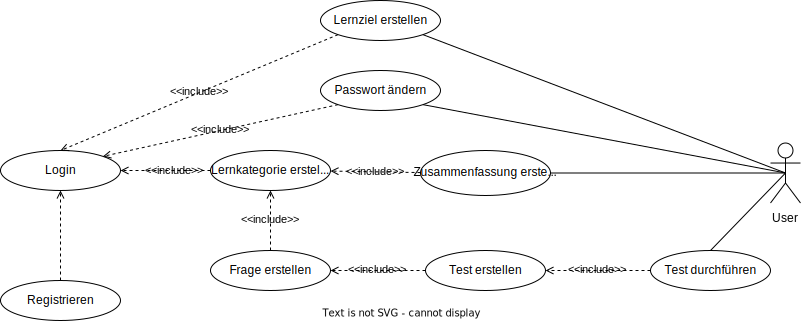
\includegraphics[width=1\textwidth]{images/diagramme/UseCase_Diagramm.png}
  \caption{Use Case Diagramm}
  \label{fig:UseCaseDiagramm}
\end{figure}
\newpage
\subsection{Use Case Beschreibung}

% Use Case Login
\begin{table}[h!]
  \begin{tabular}{p{0.2\textwidth}|p{0.74\textwidth}}
    \textbf{Name:}     & \textbf{Login}                                                                  \\ \hline
    Ziel:              & Anmelden mit bestehenden Logindaten in der App                                  \\ \hline
    Kategorie:         & Primär                                                                          \\ \hline
    Vorbedingung:      & Der Benutzer muss bereits einen Account erstellt haben                          \\ \hline
    Nachbedingung:     & Der Benutzer ist eingeloggt                                                     \\ \hline
    Fehlerfälle:       &
    \begin{minipage}[t]{\linewidth}
      Falsche Logindaten
      \strut
      \begin{itemize}
        \item Rückmeldung, dass falsche Zugangsdaten verwendet wurden
        \item Möglichkeit, das Kennwort über die E-Mail zurückzusetzen
      \end{itemize}
      Abbruch durch den Benutzer
      \begin{itemize}
        \item keine Zustandsänderung \strut
      \end{itemize}
    \end{minipage}                                                                       \\ \hline
    Akteure:           & User                                                                            \\ \hline
    Auslösendes Event: & Benutzer öffnet die App und klickt auf einloggen                                \\ \hline
    Beschreibung/
    Erweiterungen:     & Der Benutzer meldet sich an, um die verschiedenen Dienste der App zu verwenden  \\ \hline
    Alternativen:      & Benutzer kann sich registrieren, sofern die E-Mail nicht schon registriert ist. \\
  \end{tabular}
\end{table}
% Use Case Registrieren
\begin{table}[h!]
  \begin{tabular}{p{0.2\textwidth}|p{0.74\textwidth}}
    \textbf{Name:}     & \textbf{Registrieren}                                       \\ \hline
    Ziel:              & Anlegen eines neuen Accounts                                \\ \hline
    Kategorie:         & Primär                                                      \\ \hline
    Vorbedingung:      & E-Mail ist noch nicht mit einem anderen Account registriert \\ \hline
    Nachbedingung:     & Der Benutzer ist eingeloggt                                 \\ \hline
    Fehlerfälle:       &
    \begin{minipage}[t]{\linewidth}
      E-Mail bereits verwendet
      \strut
      \begin{itemize}
        \item Rückmeldung, dass E-Mail bereits verwendet wurde
      \end{itemize}
      Abbruch durch den Benutzer
      \begin{itemize}
        \item Keine Zustandsänderung
        \item Account wird nicht angelegt \strut
      \end{itemize}
    \end{minipage}                                                   \\ \hline
    Akteure:           & User                                                        \\ \hline
    Auslösendes Event: & Benutzer öffnet die App und klickt auf Registrieren.        \\ \hline
    Beschreibung/
    Erweiterungen:     & Ein Benutzer möchte einen neuen Account erstellen.          \\ \hline
    Alternativen:      & Login mit bestehendem Account.                              \\
  \end{tabular}
\end{table}
% Use Case Lernziel erstellen
\begin{table}[h!]
  \begin{tabular}{p{0.2\textwidth}|p{0.74\textwidth}}
    \textbf{Name:}     & \textbf{Lernziel erstellen}                                                                                                                                                \\ \hline
    Ziel:              & Anlegen eines neuen Lernziels                                                                                                                                              \\ \hline
    Kategorie:         & Primär                                                                                                                                                                     \\ \hline
    Vorbedingung:      &
    \begin{minipage}[t]{\linewidth}
      \strut
      \begin{itemize}
        \item User musss eingeloggt sein
        \item Lernziel mit gleichem Namen ist noch nicht erstellt \strut
      \end{itemize}
    \end{minipage}                                                                                                                                                                  \\ \hline
    Nachbedingung:     & Lernziel ist erstellt                                                                                                                                                      \\ \hline
    Fehlerfälle:       &
    \begin{minipage}[t]{\linewidth}
      Lernziel mit gleichem Namen existiert bereits
      \strut
      \begin{itemize}
        \item Rückmeldung, dass dieses Lernziel bereits existiert
      \end{itemize}
      Abbruch durch den Benutzer
      \begin{itemize}
        \item keine Zustandsänderung
        \item Lernziel wird nicht angelegt \strut
      \end{itemize}
    \end{minipage}                                                                                                                                                    \\ \hline
    Akteure:           & User                                                                                                                                                                       \\ \hline
    Auslösendes Event: & Benutzer öffnet Lernziel Reiter und klickt auf \gqq{Lernziel erstellen}                                                                                                    \\ \hline
    Beschreibung/
    Erweiterungen:     & Durch das Ausfüllen der Eingabefelder und anschließendes bestätigen, kann der User ein Lernziel erstellen. Aus sämtlichen Lernzielen wird daraufhin ein Lernplan erstellt. \\ \hline
    Alternativen:      &                                                                                                                                                                            \\
  \end{tabular}
\end{table}
% Use Case Lernkategorie erstellen
\begin{table}[H]
  \begin{tabular}{p{0.2\textwidth}|p{0.74\textwidth}}
    \textbf{Name:}     & \textbf{Lernkategorie erstellen}                                                                                                                                                                         \\ \hline
    Ziel:              & Anlegen einer neuen Lernkategorie                                                                                                                                                                   \\ \hline
    Kategorie:         & Primär                                                                                                                                                                                              \\ \hline
    Vorbedingung:      &
    \begin{minipage}[t]{\linewidth}
      \strut
      \begin{itemize}
        \item User musss eingeloggt sein
        \item Lernkategorie mit gleichem Namen ist noch nicht erstellt \strut
      \end{itemize}
    \end{minipage}                                                                                                                                                                                           \\ \hline
    Nachbedingung:     & Lernkategorie ist erstellt                                                                                                                                                                          \\ \hline
    Fehlerfälle:       &
    \begin{minipage}[t]{\linewidth}
      Lernkategorie mit gleichem Namen existiert bereits
      \strut
      \begin{itemize}
        \item Rückmeldung, dass diese Lernkategorie bereits existiert
      \end{itemize}
      Abbruch durch den Benutzer
      \begin{itemize}
        \item keine Zustandsänderung
        \item Lernkategorie wird nicht angelegt \strut
      \end{itemize}
    \end{minipage}                                                                                                                                                                        \\ \hline
    Akteure:           & User                                                                                                                                                                                                \\ \hline
    Auslösendes Event: & Benutzer öffnet Lernkategorie Reiter und klickt auf \gqq{Lernkategorie erstellen}                                                                                                                   \\ \hline
    Beschreibung/
    Erweiterungen:     & Durch das Ausfüllen der Eingabefelder und anschließendes bestätigen, kann der User eine Lernkategorie erstellen. In einer Lernkategorie können Zusammenfassungen, Fragen und Tests erstellt werden. \\ \hline
    Alternativen:      &                                                                                                                                                                                                     \\
  \end{tabular}
\end{table}
% Use Case Zusammenfassung erstellen
\begin{table}[h!]
  \begin{tabular}{p{0.2\textwidth}|p{0.74\textwidth}}
    \textbf{Name:}     & \textbf{Zusammenfassung erstellen}                                                                                                                                                          \\ \hline
    Ziel:              & Anlegen einer neuen Zusammenfassung                                                                                                                                                         \\ \hline
    Kategorie:         & Primär                                                                                                                                                                                      \\ \hline
    Vorbedingung:      &
    \begin{minipage}[t]{\linewidth}
      \strut
      \begin{itemize}
        \item User musss eingeloggt sein
        \item Zusammenfassung mit gleichem Namen ist noch nicht in der gleichen Lernkategorie
              erstellt \strut
      \end{itemize}
    \end{minipage}                                                                                                                                                                                   \\ \hline
    Nachbedingung:     & Zusammenfassung für Lernkategorie ist erstellt                                                                                                                                              \\ \hline
    Fehlerfälle:       &
    \begin{minipage}[t]{\linewidth}
      Zusammenfassung mit gleichem Namen existiert bereits in dieser Lernkategorie
      \strut
      \begin{itemize}
        \item Rückmeldung, dass diese Zusammenfassung bereits existiert
      \end{itemize}
      Abbruch durch den Benutzer
      \begin{itemize}
        \item keine Zustandsänderung
        \item Zusammenfassung wird nicht angelegt \strut
      \end{itemize}
    \end{minipage}                                                                                                                                      \\ \hline
    Akteure:           & User                                                                                                                                                                                        \\ \hline
    Auslösendes Event: & Benutzer öffnet eine Lernkategorie, klickt auf \gqq{Zusammenfassungen} und danach auf \gqq{Zusammenfassung erstellen}                                                                       \\ \hline
    Beschreibung/
    Erweiterungen:     & Durch das Ausfüllen der Eingabefelder und anschließendes bestätigen, kann der User eine Zusammenfassung erstellen. In einer Zusammenfassung können Inhalte eingefügt und formatiert werden. \\ \hline
    Alternativen:      &                                                                                                                                                                                             \\
  \end{tabular}
\end{table}
% Use Case Frage erstellen
\begin{table}[H]
  \begin{tabular}{p{0.2\textwidth}|p{0.74\textwidth}}
    \textbf{Name:}     & \textbf{Frage erstellen}                                                                                                                                                                                                                                               \\ \hline
    Ziel:              & Anlegen einer neuen Frage                                                                                                                                                                                                                                              \\ \hline
    Kategorie:         & Primär                                                                                                                                                                                                                                                                 \\ \hline
    Vorbedingung:      &
    \begin{minipage}[t]{\linewidth}
      \strut
      \begin{itemize}
        \item User musss eingeloggt sein
        \item Frage mit gleichem Index ist noch nicht in der gleichen Lernkategorie erstellt
              \strut
      \end{itemize}
    \end{minipage}                                                                                                                                                                                                                                                              \\ \hline
    Nachbedingung:     & Frage für Lernkategorie ist erstellt                                                                                                                                                                                                                                   \\ \hline
    Fehlerfälle:       &
    \begin{minipage}[t]{\linewidth}
      Frage mit gleichem Namen existiert bereits in dieser Lernkategorie
      \strut
      \begin{itemize}
        \item Rückmeldung, dass Frage mit gleicher Bezeichnung bereits existiert
      \end{itemize}
      Abbruch durch den Benutzer
      \begin{itemize}
        \item keine Zustandsänderung
        \item Frage wird nicht angelegt \strut
      \end{itemize}
    \end{minipage}                                                                                                                                                                                                                           \\ \hline
    Akteure:           & User                                                                                                                                                                                                                                                                   \\ \hline
    Auslösendes Event: & Benutzer öffnet eine Lernkategorie, klickt auf \gqq{Tests / Fragen} und danach auf \gqq{Frage erstellen}                                                                                                                                                               \\ \hline
    Beschreibung/
    Erweiterungen:     & Durch das Ausfüllen der Eingabefelder und anschließendes bestätigen, kann der User eine Frage erstellen. Eine Frage kann unterschiedliche Vorlagen (beispielsweise Karteikarte) besitzen, jedoch gibt es immer eine Meldung (Text der Frage) und eine gültige Antwort. \\ \hline
    Alternativen:      &                                                                                                                                                                                                                                                                        \\
  \end{tabular}
\end{table}
% Use Case Test erstellen
\begin{table}[H]
  \begin{tabular}{p{0.2\textwidth}|p{0.74\textwidth}}
    \textbf{Name:}     & \textbf{Test erstellen}                                                                                                                                                                                                                                                                           \\ \hline
    Ziel:              & Anlegen eines neuen Tests                                                                                                                                                                                                                                                                         \\ \hline
    Kategorie:         & Primär                                                                                                                                                                                                                                                                                            \\ \hline
    Vorbedingung:      &
    \begin{minipage}[t]{\linewidth}
      \strut
      \begin{itemize}
        \item User musss eingeloggt sein
        \item Test mit gleichem Namen ist noch nicht in der gleichen Lernkategorie erstellt
              \strut
      \end{itemize}
    \end{minipage}                                                                                                                                                                                                                                                                                         \\ \hline
    Nachbedingung:     & Test für Lernkategorie ist erstellt                                                                                                                                                                                                                                                               \\ \hline
    Fehlerfälle:       &
    \begin{minipage}[t]{\linewidth}
      Test mit gleichem Namen existiert bereits in dieser Lernkategorie
      \strut
      \begin{itemize}
        \item Rückmeldung, dass Test mit gleicher Bezeichnung bereits existiert
      \end{itemize}
      Abbruch durch den Benutzer
      \begin{itemize}
        \item keine Zustandsänderung
        \item Test wird nicht angelegt \strut
      \end{itemize}
    \end{minipage}                                                                                                                                                                                                                                                       \\ \hline
    Akteure:           & User                                                                                                                                                                                                                                                                                              \\ \hline
    Auslösendes Event: & Benutzer öffnet eine Lernkategorie, klickt auf \gqq{Tests / Fragen} und danach auf \gqq{Test erstellen}                                                                                                                                                                                           \\ \hline
    Beschreibung/
    Erweiterungen:     & Durch das Ausfüllen der Eingabefelder und anschließendes bestätigen, kann der User einen Test erstellen. Eine Test kann mehrere Fragen besitzen. Wenn ein Test gestartet wird, bekommt der User nach abschließen des Tests eine Meldung, wie viele und welche Fragen er richtig beantwortet hast. \\ \hline
    Alternativen:      &                                                                                                                                                                                                                                                                                                   \\
  \end{tabular}
\end{table}
\newpage

\subsection{Datenbankstruktur}
\subsubsection{Datenbankmodell}
\begin{figure}[H]
  \centering
  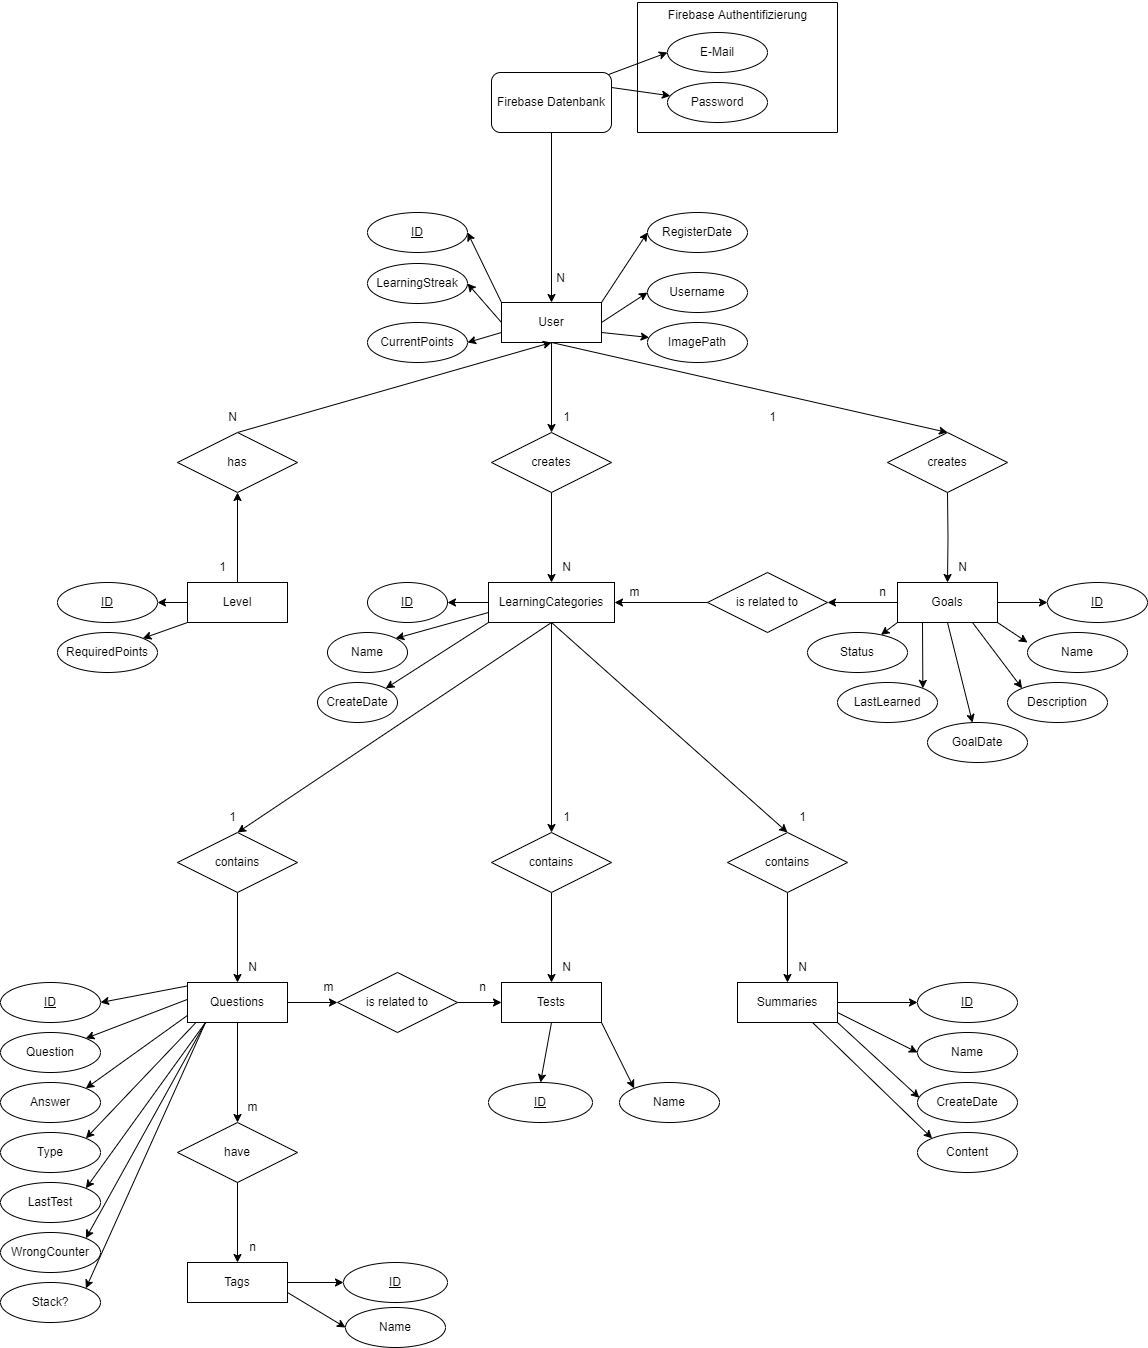
\includegraphics[width=1\textwidth]{images/LearnAheadDatenbankstruktur.png}
  \caption{LearnAhead Datenbankstruktur}
  \label{fig:LearnAheadDatenbankstruktur}
\end{figure}\noindent
\subsubsection{Data Dictionary}
\underline{\textbf{User}}
\begin{table}[H]
  \centering
  \resizebox{\columnwidth}{!}{%
    \begin{tabular}{c|c|c|c|c|c|l}
      \textbf{Attribut}  &
      \textbf{Datentyp}  &
      \textbf{Länge}     &
      \textbf{Null}      &
      \textbf{Default}   &
      \textbf{Schlüssel} &
      \textbf{Beschreibung}                                                                                                                                                         \\ \hline
      ID                 &
      string             &
      -                  &
      Nein               &
      -                  &
      P                  &
      \\ \hline
      Username           &
      string             &
      -                  &
      Nein               &
      -                  &
      -                  &
      Der Benutzername des Nutzers                                                                                                                                                  \\ \hline
      E-Mail             &
      string             &
      -                  &
      Nein               &
      -                  &
      -                  &
      Die E-Mail-Adresse des Nutzers                                                                                                                                                \\ \hline
      Password           &
      string             &
      -                  &
      Nein               &
      -                  &
      -                  &
      Das Passwort des Nutzers                                                                                                                                                      \\ \hline
      ProfileImageURL    &
      string             &
      -                  &
      Ja                 &
      Null               &
      -                  &
      \begin{tabular}[c]{@{}l@{}}Der Link des Profilbilds welches\\ im Firebase Storage gespeichert\\ ist\end{tabular}                                                              \\ \hline
      RegisterDate       &
      timestamp          &
      -                  &
      Nein               &
      -                  &
      -                  &
      \begin{tabular}[c]{@{}l@{}}Das Datum an dem sich der \\ Nutzer registriert hat.\end{tabular}                                                                                  \\ \hline
      LearningStreak     &
      number             &
      -                  &
      Ja                 &
      0                  &
      -                  &
      \begin{tabular}[c]{@{}l@{}}Dies gibt die Anzahl an, wie viele\\ Tage der Nutzer aufeinander \\ gelernt hat.\end{tabular}                                                      \\ \hline
      AchievedGoals      &
      number             &
      -                  &
      Ja                 &
      0                  &
      -                  &
      \begin{tabular}[c]{@{}l@{}}Dies gibt die Anzahl an, wie viele\\ Lernziel der Nutzer erreicht hat.\end{tabular}                                                                \\ \hline
      CurrentPoints      &
      number             &
      -                  &
      Ja                 &
      0                  &
      -                  &
      \begin{tabular}[c]{@{}l@{}}Die aktuelle Level Punkte des\\ Nutzers\end{tabular}                                                                                               \\ \hline
      LearningCategories &
      map                &
      -                  &
      Ja                 &
      Null               &
      -                  &
      \begin{tabular}[c]{@{}l@{}}Dies ist eine gemappte Liste zu\\ der Tabelle LearningCategories, \\ wo alle Lernkategorien drin sind,\\ die der Nutzer erstellt hat.\end{tabular} \\ \hline
      Goals              &
      map                &
      -                  &
      Ja                 &
      Null               &
      -                  &
      \begin{tabular}[c]{@{}l@{}}Dies ist eine gemappte Liste zu \\ der Tabelle Goals, wo alle\\ Lernziele drin sind, die der\\ Nutzer erstellt hat.\end{tabular}
    \end{tabular}%
  }
\end{table}
\underline{\textbf{Level}}
\begin{table}[H]
  \centering
  \resizebox{\columnwidth}{!}{%
  \begin{tabular}{c|c|c|c|c|c|l}
  \textbf{Attribut} &
    \textbf{Datentyp} &
    \textbf{Länge} &
    \textbf{Null} &
    \textbf{Default} &
    \textbf{Schlüssel} &
    \textbf{Beschreibung} \\ \hline
  ID &
    string &
    - &
    Nein &
    - &
    P &
     \\ \hline
  RequiredPoints & number & - & Nein & - & - & \begin{tabular}[c]{@{}l@{}}Dies gibt die benötigten\\ Punkte für das spezielle\\ Level an\end{tabular} \\ \hline
  Level &
    number &
    - &
    Nein &
    - &
    - &
    \begin{tabular}[c]{@{}l@{}}Dies gibt das spezielle \\ Level anhand der Punkte an\end{tabular}
  \end{tabular}%
  }
  \end{table}
\newpage
\underline{\textbf{Goal}}
\begin{table}[H]
  \centering
  \resizebox{\columnwidth}{!}{%
    \begin{tabular}{c|c|c|c|c|c|l}
      \textbf{Attribut}                                          &
      \textbf{Datentyp}                                          &
      \textbf{Länge}                                             &
      \textbf{Null}                                              &
      \textbf{Default}                                           &
      \textbf{Schlüssel}                                         &
      \textbf{Beschreibung}                                                                                                                                       \\ \hline
      ID                                                         &
      string                                                     &
      -                                                          &
      Nein                                                       &
      -                                                          &
      P                                                          &
      \\ \hline
      Name                                                       &
      string                                                     &
      -                                                          &
      Nein                                                       &
      -                                                          &
      -                                                          &
      Der Name des Lernziels                                                                                                                                      \\ \hline
      Description                                                &
      string                                                     &
      -                                                          &
      Ja                                                         &
      Null                                                       &
      -                                                          &
      \begin{tabular}[c]{@{}l@{}}Dies soll als Beschreibung des\\ Lernziels gelten. Hier können\\ z.B. die relevanten Themen\\ aufgelistet werden.\end{tabular}   \\ \hline
      Status                                                     &
      string                                                     &
      -                                                          &
      Ja                                                         &
      ToDo                                                       &
      -                                                          &
      \begin{tabular}[c]{@{}l@{}}Dies gibt den aktuellen Status\\ des Lernziels an.\\ Es gibt die folgende Status:\\ - ToDo\\ - In Progress\\ - Done\end{tabular} \\ \hline
      StartDate                                                  &
      timestamp                                                  &
      -                                                          &
      Ja                                                         &
      \begin{tabular}[c]{@{}c@{}}Server\\ Timestamp\end{tabular} &
      -                                                          &
      \begin{tabular}[c]{@{}l@{}}Dies gibt an, wann das \\ Lernziel startet\end{tabular}                                                                          \\ \hline
      EndDate                                                    &
      timestamp                                                  &
      -                                                          &
      Nein                                                       &
      -                                                          &
      -                                                          &
      \begin{tabular}[c]{@{}l@{}}Dies gibt an, bis wann das\\ Lernziel abgeschlossen sein\\ soll\end{tabular}                                                     \\ \hline
      LastLearned                                                &
      timestamp                                                  &
      -                                                          &
      Ja                                                         &
      Null                                                       &
      -                                                          &
      \begin{tabular}[c]{@{}l@{}}Dies gibt, wann das Lernziel\\ das letzte mal gelernt wurde.\end{tabular}
    \end{tabular}%
  }
\end{table}
\newpage
% Data Dicitonary Learning Category Table
\underline{\textbf{LearningCategory}}
\begin{table}[H]
  \centering
  \resizebox{\columnwidth}{!}{%
    \begin{tabular}{c|c|c|c|c|c|l}
      \textbf{Attribut}                                          &
      \textbf{Datentyp}                                          &
      \textbf{Länge}                                             &
      \textbf{Null}                                              &
      \textbf{Default}                                           &
      \textbf{Schlüssel}                                         &
      \textbf{Beschreibung}                                                                                                                                                \\ \hline
      ID                                                         &
      string                                                     &
      -                                                          &
      Nein                                                       &
      -                                                          &
      P                                                          &
      \\ \hline
      Name                                                       &
      string                                                     &
      -                                                          &
      Nein                                                       &
      -                                                          &
      -                                                          &
      Der Name der Lernkategorie                                                                                                                                           \\ \hline
      CreateDate                                                 &
      timestamp                                                  &
      -                                                          &
      Ja                                                         &
      \begin{tabular}[c]{@{}c@{}}Server\\ Timestamp\end{tabular} &
      -                                                          &
      \begin{tabular}[c]{@{}l@{}}Dies gibt an, wann die \\ Lernkategorie erstellt wurde\end{tabular}                                                                       \\ \hline
      Goals                                                      &
      map                                                        &
      -                                                          &
      Ja                                                         &
      Null                                                       &
      -                                                          &
      \begin{tabular}[c]{@{}l@{}}Dies ist eine gemappte Liste zu\\ der Tabelle Goal,\\ wo alle Lernziele drin sind,\\ die der Nutzer erstellt hat.\end{tabular}            \\ \hline
      Questions                                                  &
      map                                                        &
      -                                                          &
      Ja                                                         &
      Null                                                       &
      -                                                          &
      \begin{tabular}[c]{@{}l@{}}Dies ist eine gemappte Liste zu\\ der Tabelle Question, wo alle \\ Fragen drin sind, die der \\ Nutzer erstellt hat.\end{tabular}         \\ \hline
      Summaries                                                  &
      map                                                        &
      -                                                          &
      Ja                                                         &
      Null                                                       &
      -                                                          &
      \begin{tabular}[c]{@{}l@{}}Dies ist eine gemappte Liste zu\\ der Tabelle Summary, wo alle\\ Zusammenfassungen drin sind,\\ die der Nutzer erstellt hat.\end{tabular} \\ \hline
      Tests                                                      &
      map                                                        &
      -                                                          &
      Ja                                                         &
      Null                                                       &
      -                                                          &
      \begin{tabular}[c]{@{}l@{}}Dies ist eine gemappte Liste zu\\ der Tabelle Test, wo alle Tests\\ drin sind, die der Nutzer\\ erstellt hat.\end{tabular}
    \end{tabular}%
  }
\end{table}
\underline{\textbf{Summary}}
\begin{table}[H]
  \centering
  \resizebox{\columnwidth}{!}{%
  \begin{tabular}{c|c|c|c|c|c|l}
  \textbf{Attribut} &
    \textbf{Datentyp} &
    \textbf{Länge} &
    \textbf{Null} &
    \textbf{Default} &
    \textbf{Schlüssel} &
    \textbf{Beschreibung} \\ \hline
  ID &
    string &
    - &
    Nein &
    - &
    P &
     \\ \hline
  Name &
    string &
    - &
    Nein &
    - &
    - &
    \begin{tabular}[c]{@{}l@{}}Dies ist der Name einer\\ Zusammenfassung\end{tabular} \\ \hline
  CreateDate &
    timestamp &
    - &
    Nein &
    - &
    - &
    \begin{tabular}[c]{@{}l@{}}Dies ist das Erstelldatum\\ einer Zusammenfassung\end{tabular} \\ \hline
  Content & string & - & Ja & Null & - & \begin{tabular}[c]{@{}l@{}}Dies ist ist der Inhalt einer\\ Zusammenfassung im \\ Raw-Format\end{tabular}
  \end{tabular}%
  }
  \end{table}
  \newpage
  \underline{\textbf{Test}}
  % Please add the following required packages to your document preamble:
% \usepackage{graphicx}
\begin{table}[H]
  \centering
  \resizebox{\columnwidth}{!}{%
  \begin{tabular}{c|c|c|c|c|c|l}
  \textbf{Attribut} &
    \textbf{Datentyp} &
    \textbf{Länge} &
    \textbf{Null} &
    \textbf{Default} &
    \textbf{Schlüssel} &
    \textbf{Beschreibung} \\ \hline
  ID &
    string &
    - &
    Nein &
    - &
    P &
     \\ \hline
  Name &
    string &
    - &
    Nein &
    - &
    - &
    \begin{tabular}[c]{@{}l@{}}Dies ist der Name eines\\ Tests\end{tabular} \\ \hline
  Questions &
    map &
    - &
    Ja &
    Null &
    - &
    \begin{tabular}[c]{@{}l@{}}Dies ist eine gemappte Liste zu\\ der Tabelle Question, wo alle\\ Fragen drin sind, die der\\ Nutzer erstellt hat.\end{tabular} \\ \hline
  \end{tabular}%
  }
  \end{table}
  \underline{\textbf{Question}}
  % Please add the following required packages to your document preamble:
% \usepackage{graphicx}
\begin{table}[H]
  \centering
  \resizebox{\columnwidth}{!}{%
  \begin{tabular}{c|c|c|c|c|c|l}
  \textbf{Attribut} &
    \textbf{Datentyp} &
    \textbf{Länge} &
    \textbf{Null} &
    \textbf{Default} &
    \textbf{Schlüssel} &
    \textbf{Beschreibung} \\ \hline
  ID &
    string &
    - &
    Nein &
    - &
    P &
     \\ \hline
  Question &
    string &
    - &
    Nein &
    - &
    - &
    Die Frage der Frage \\ \hline
  Answer &
    string &
    - &
    Nein &
    - &
    - &
    Die Antwort auf die Frage \\ \hline
  Type &
    number &
    - &
    Nein &
    - &
    - &
    \begin{tabular}[c]{@{}l@{}}Dies soll den Typ einer Frage \\ angeben:\\ z.B.\\ Type = 0 = Karteikarten\\ Type = 1 = Multiple Choice\end{tabular} \\ \hline
  LastTest &
    bool &
    - &
    Ja &
    Null &
    - &
    \begin{tabular}[c]{@{}l@{}}Dies gibt an ob die Frage beim \\ letzten Mal richtig beantwortet \\ wurde\end{tabular} \\ \hline
  WrongCounter &
    number &
    - &
    Ja &
    0 &
    - &
    \begin{tabular}[c]{@{}l@{}}Dies gibt an wie oft die Frage\\ hintereinander falsch beantwortet\\ wurde. Wird diese dann richtig\\ beantwortet setzt sich der Counter\\ auf 0 zurück\end{tabular} \\ \hline
  Tags &
    map &
    - &
    Nein &
     &
    - &
    \begin{tabular}[c]{@{}l@{}}Dies ist eine gemappte Liste zu\\ der Tabelle Tags, wo alle Tags\\ drin sind, die der Nutzer erstellt\\ hat.\end{tabular} \\ \hline
  \end{tabular}%
  }
  \end{table}
  \underline{\textbf{Tag}}
  % Please add the following required packages to your document preamble:
% \usepackage{graphicx}
\begin{table}[H]
  \centering
  \resizebox{\columnwidth}{!}{%
  \begin{tabular}{c|c|c|c|c|c|l}
  \textbf{Attribut} & \textbf{Datentyp} & \textbf{Länge} & \textbf{Null} & \textbf{Default} & \textbf{Schlüssel} & \textbf{Beschreibung} \\ \hline
  ID                & string            & -              & Nein          & -                & P                  &                       \\ \hline
  Name              & string            & -              & Nein          & -                & -                  & Der Name des Tags     \\ \hline
  \end{tabular}%
  }
  \end{table}
\subsection{HMI}

\subsubsection{Seitenhirarchie}
Innerhalb der Seitenhierarchie wird dargestellt, wie man in der App navigieren
kann.
\begin{figure}[H]
  \centering
  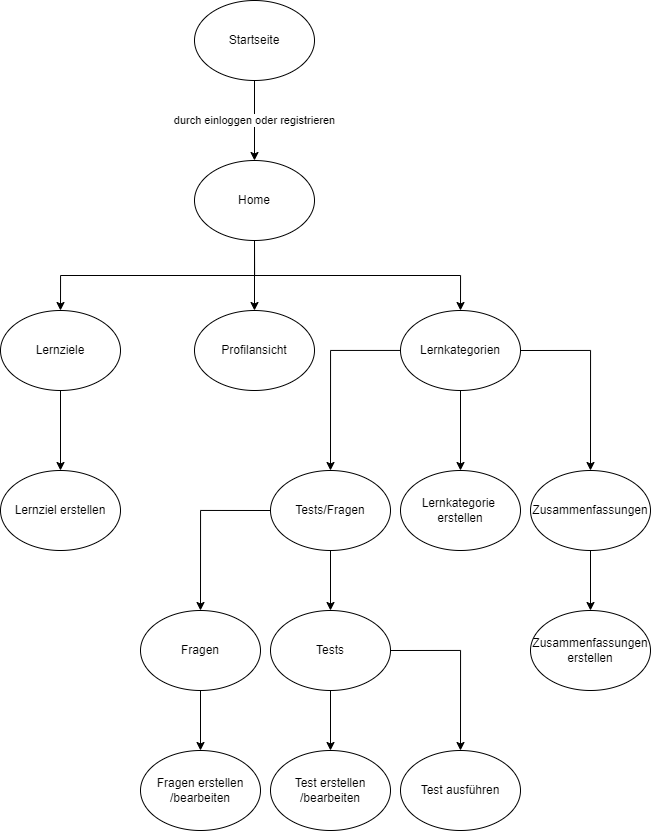
\includegraphics[width=0.8\textwidth]{images/diagramme/Seitenhierarchie.png}
  \caption{Die Seitenhierarchie in LearnAhead}
  \label{fig:UseCaseDiagramm1}
\end{figure}

\newpage
\subsubsection{UI-Mockups}

\begin{figure}[htbp]
  \centering
  \begin{subfigure}[b]{0.45\linewidth}
    \centering
    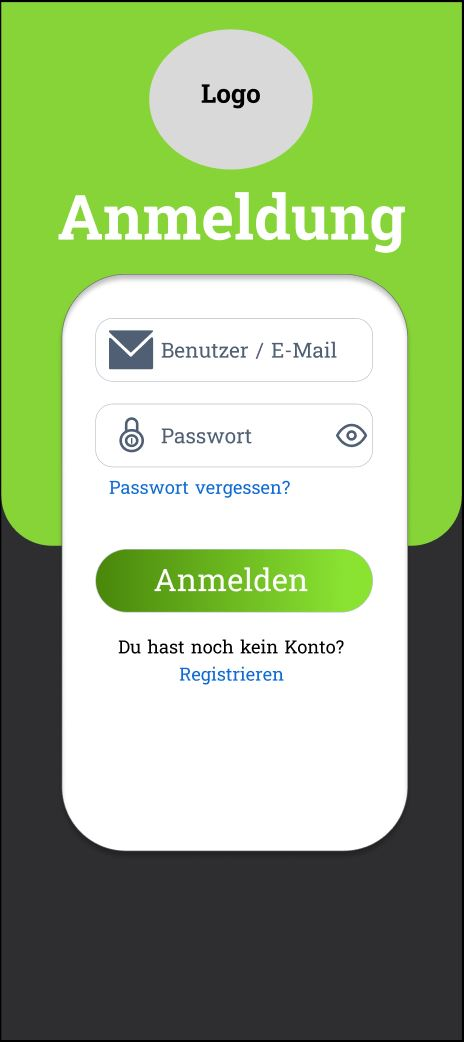
\includegraphics[width=\linewidth]{images/Mockups/Login.JPG}
    \caption{Login-Screen}
    \label{fig:login-screen}
  \end{subfigure}
  \hfill
  \begin{subfigure}[b]{0.45\linewidth}
    \centering
    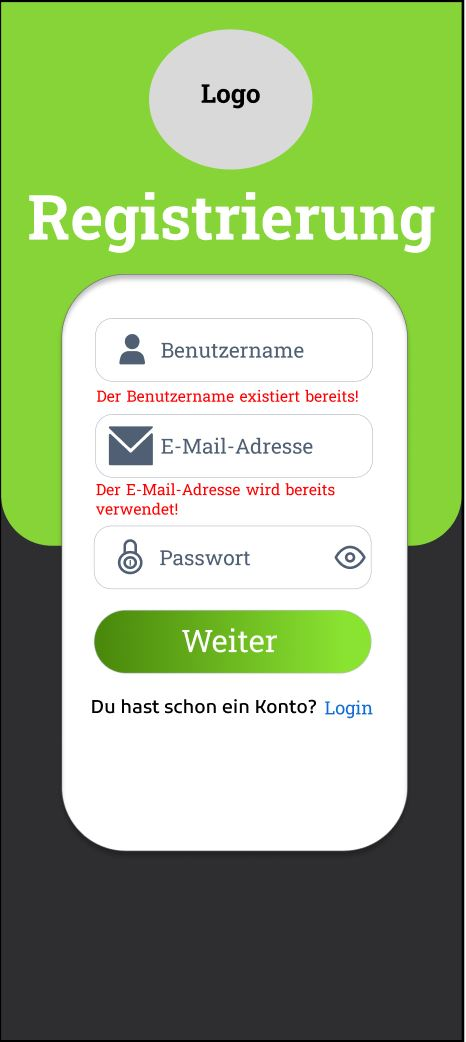
\includegraphics[width=\linewidth]{images/Mockups/Registrierung.JPG}
    \caption{Registrierung}
    \label{fig:registrierung}
  \end{subfigure}
  \caption{Login und Registrierung}
\end{figure}

\newpage

\begin{figure}[htbp]
  \centering
  \begin{subfigure}[b]{0.45\linewidth}
    \centering
    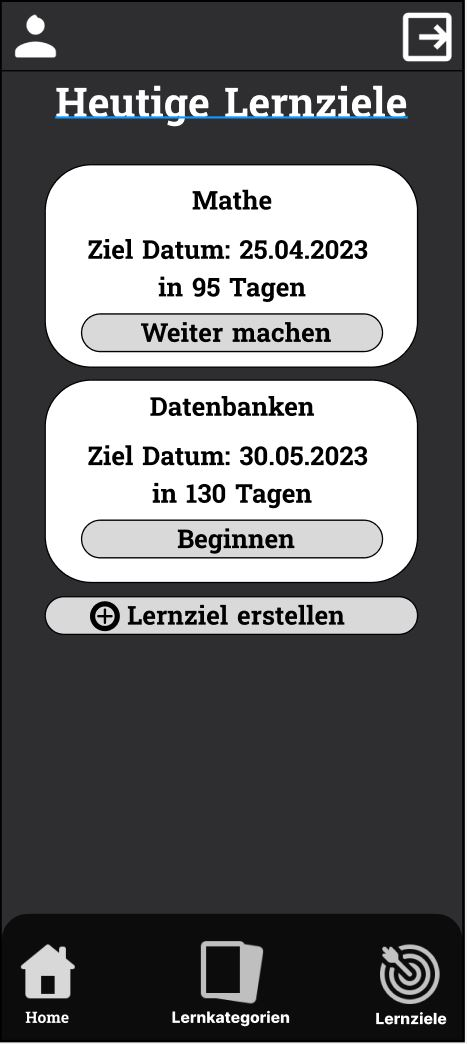
\includegraphics[width=\linewidth]{images/Mockups/Home.JPG}
    \caption{Home-Screen}
    \label{fig:home-screen}
  \end{subfigure}
  \hfill
  \begin{subfigure}[b]{0.45\linewidth}
    \centering
    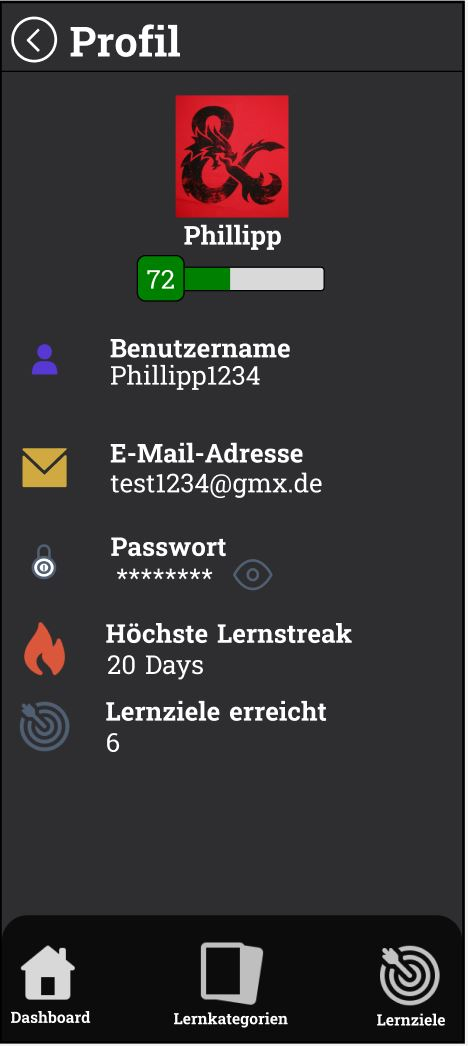
\includegraphics[width=\linewidth]{images/Mockups/Profile.JPG}
    \caption{Profilansicht}
    \label{fig:profilansicht}
  \end{subfigure}
  \caption{Home-Screen and Profilansicht}
\end{figure}

\newpage

\begin{figure}[htbp]
  \centering
  \begin{subfigure}[b]{0.45\linewidth}
    \centering
    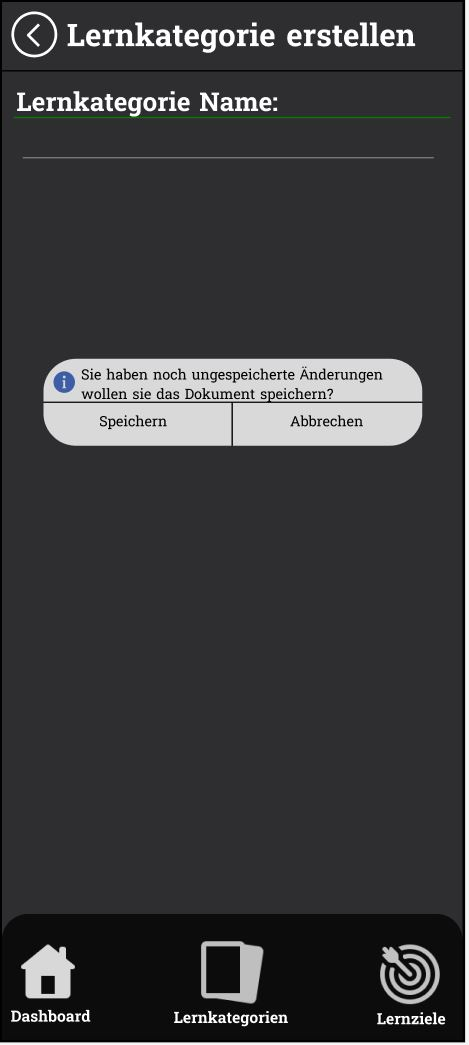
\includegraphics[width=\linewidth]{images/Mockups/createLernkategorie.JPG}
    \caption{Erstellen einer Lernkategorie}
    \label{fig:lernkategorie-create}
  \end{subfigure}
  \hfill
  \begin{subfigure}[b]{0.45\linewidth}
    \centering
    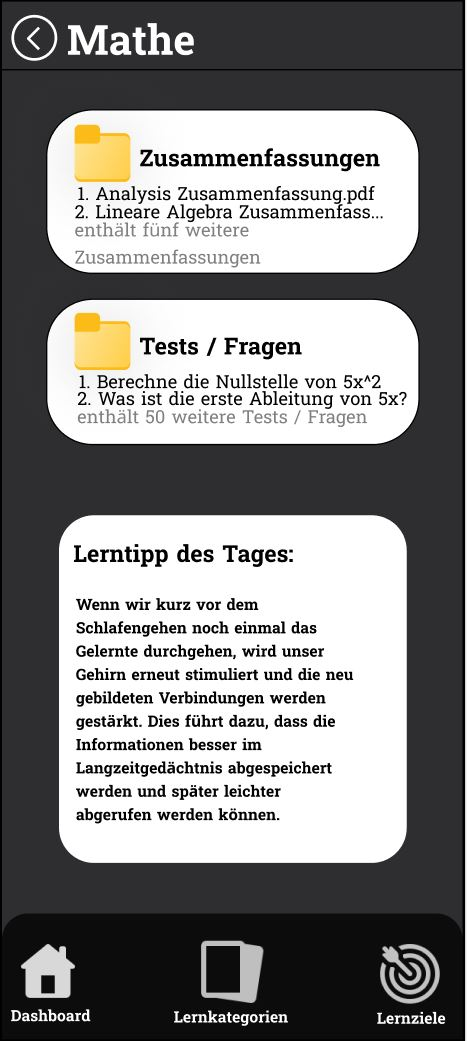
\includegraphics[width=\linewidth]{images/Mockups/Lernkategorie.JPG}
    \caption{Ansicht Lernkategorien}
    \label{fig:lernkategorie-ansicht}
  \end{subfigure}
  \caption{Erstellen einer Lernkategorie and Ansicht Lernkategorien}
  \label{fig:lernkategorie}
\end{figure}

\newpage

\begin{figure}[htbp]
  \centering
  \begin{subfigure}[b]{0.45\linewidth}
    \centering
    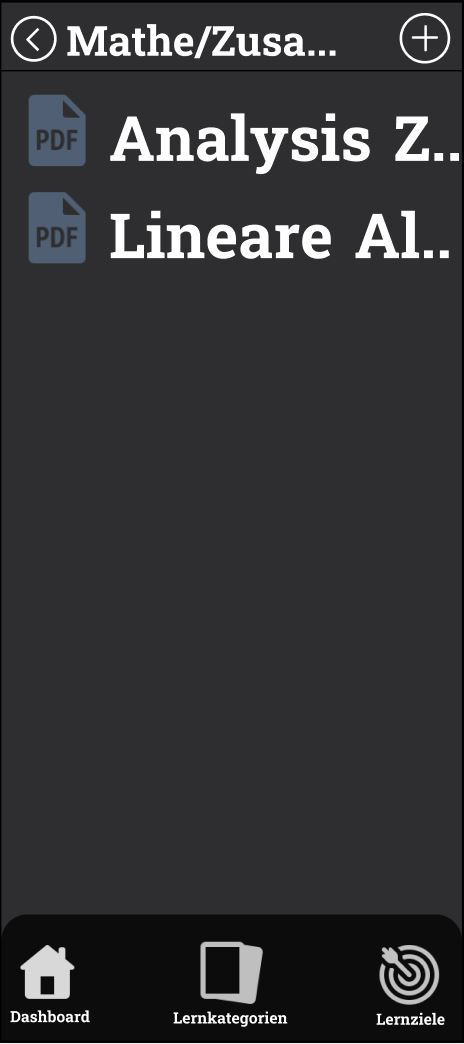
\includegraphics[width=\linewidth]{images/Mockups/Summaries.JPG}
    \caption{Ansicht Zusammenfassungen}
    \label{fig:zusammenfassungen-ansicht}
  \end{subfigure}
  \hfill
  \begin{subfigure}[b]{0.45\linewidth}
    \centering
    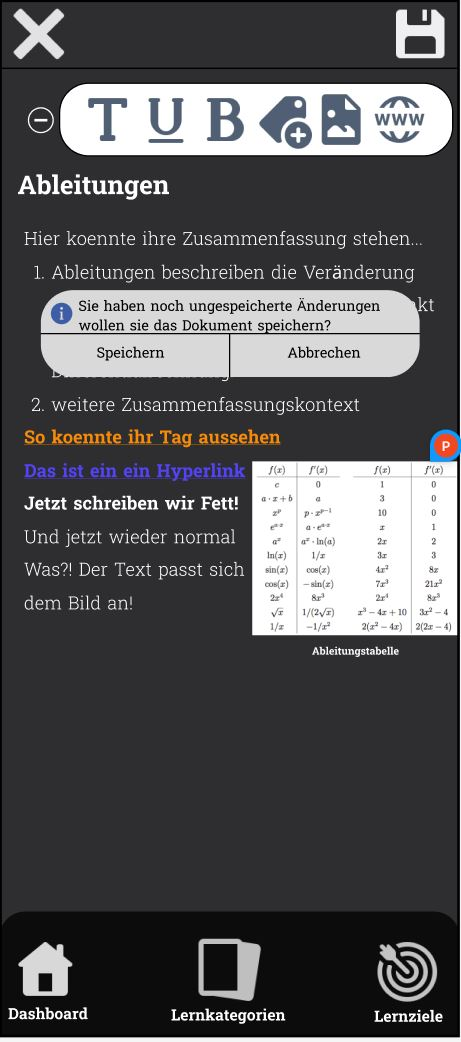
\includegraphics[width=\linewidth]{images/Mockups/Summaries_Look.JPG}
    \caption{Erstellen einer Zusammenfassung}
    \label{fig:zusammenfassungen-erstellen}
  \end{subfigure}
  \caption{Ansicht Zusammenfassungen and Erstellen einer Zusammenfassung}
  \label{fig:zusammenfassungen}
\end{figure}

\newpage

\begin{figure}[htbp]
  \centering
  \begin{subfigure}[b]{0.45\linewidth}
    \centering
    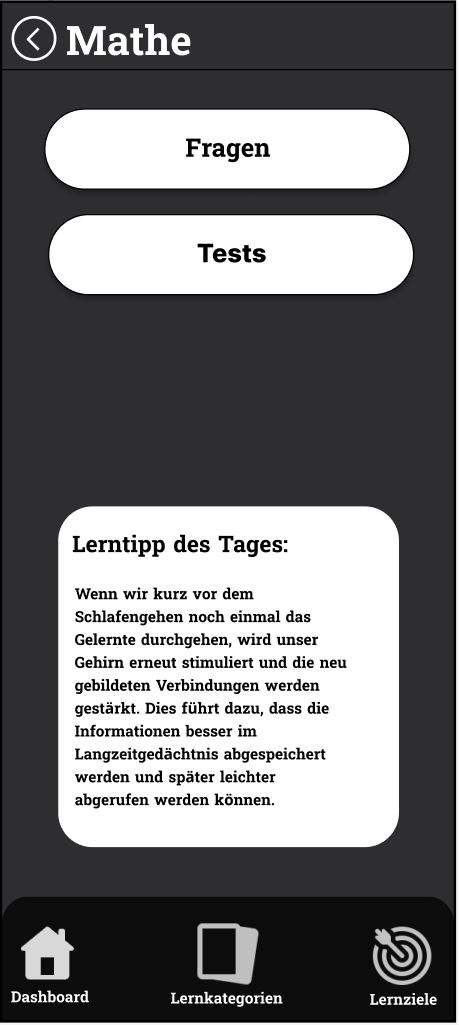
\includegraphics[width=\linewidth]{images/Mockups/FragenTests.JPG}
    \caption{Ansicht Fragen und Tests}
    \label{fig:fragen-tests-ansicht}
  \end{subfigure}
  \hfill
  \begin{subfigure}[b]{0.45\linewidth}
    \centering
    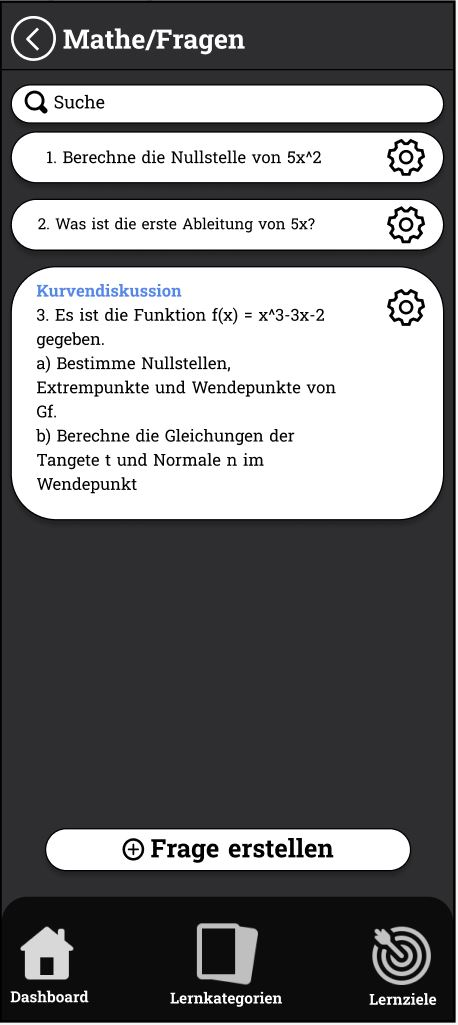
\includegraphics[width=\linewidth]{images/Mockups/Fragen.JPG}
    \caption{Ansicht Fragen}
    \label{fig:fragen-ansicht}
  \end{subfigure}
  \caption{Ansicht Fragen und Tests and Ansicht Fragen}
  \label{fig:fragen-tests}
\end{figure}

\newpage

\begin{figure}[htbp]
  \centering
  \begin{subfigure}[b]{0.45\linewidth}
    \centering
    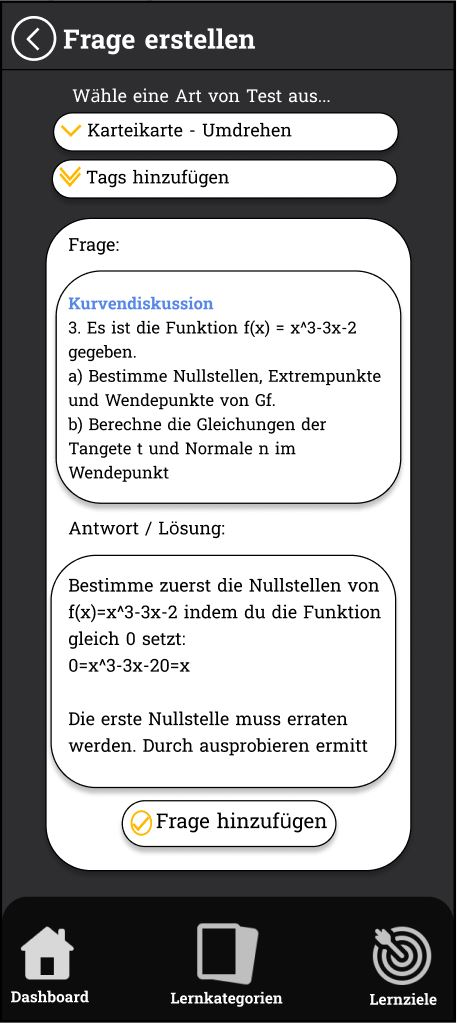
\includegraphics[width=\linewidth]{images/Mockups/FrageErstellen.JPG}
    \caption{Erstellen einer Frage}
    \label{fig:frage-erstellen}
  \end{subfigure}
  \hfill
  \begin{subfigure}[b]{0.45\linewidth}
    \centering
    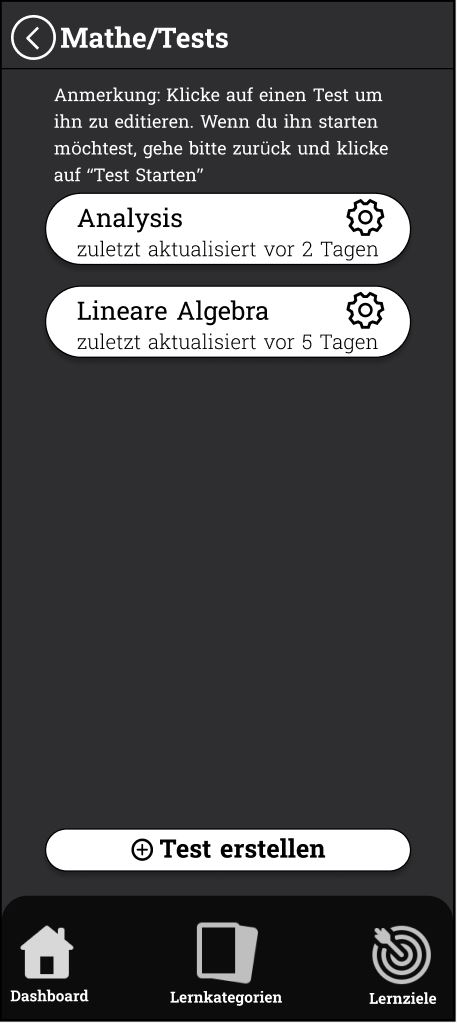
\includegraphics[width=\linewidth]{images/Mockups/Tests.JPG}
    \caption{Ansichts Tests}
    \label{fig:tests-ansicht}
  \end{subfigure}
  \caption{Erstellen einer Frage and Ansichts Tests}
  \label{fig:frage-tests}
\end{figure}

\newpage

\begin{figure}[htbp]
  \centering
  \begin{subfigure}[b]{0.45\linewidth}
    \centering
    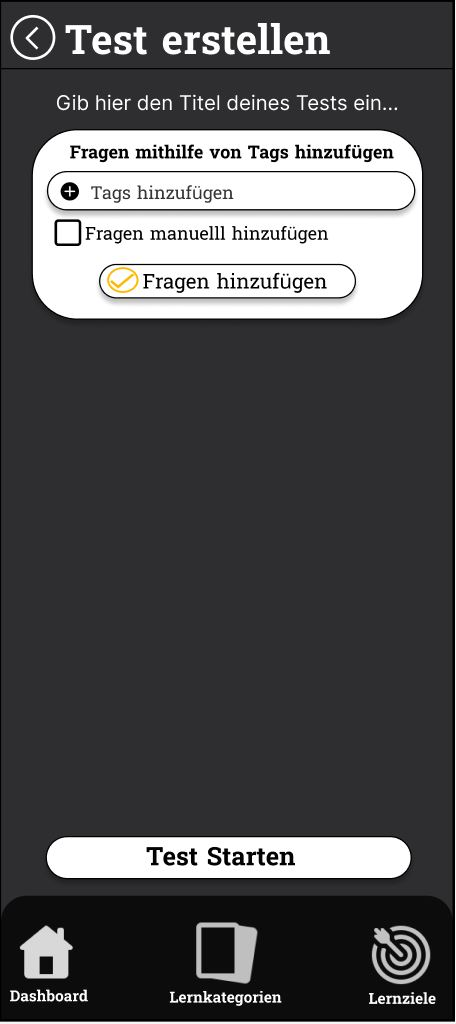
\includegraphics[width=\linewidth]{images/Mockups/TestErstellen.JPG}
    \caption{Erstellen eines Tests}
    \label{fig:test-erstellen}
  \end{subfigure}
  \hfill
  \begin{subfigure}[b]{0.45\linewidth}
    \centering
    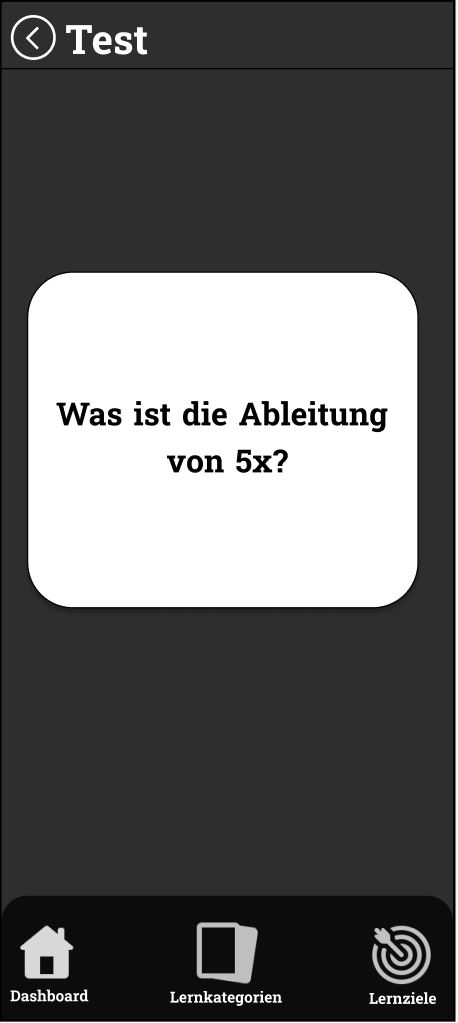
\includegraphics[width=\linewidth]{images/Mockups/TestFrage.JPG}
    \caption{Ansicht einer Frage innerhalb eines Tests}
    \label{fig:test-frage}
  \end{subfigure}
  \caption{Test}
\end{figure}

\newpage

\begin{figure}[htbp]
  \centering
  \begin{subfigure}[b]{0.45\linewidth}
    \centering
    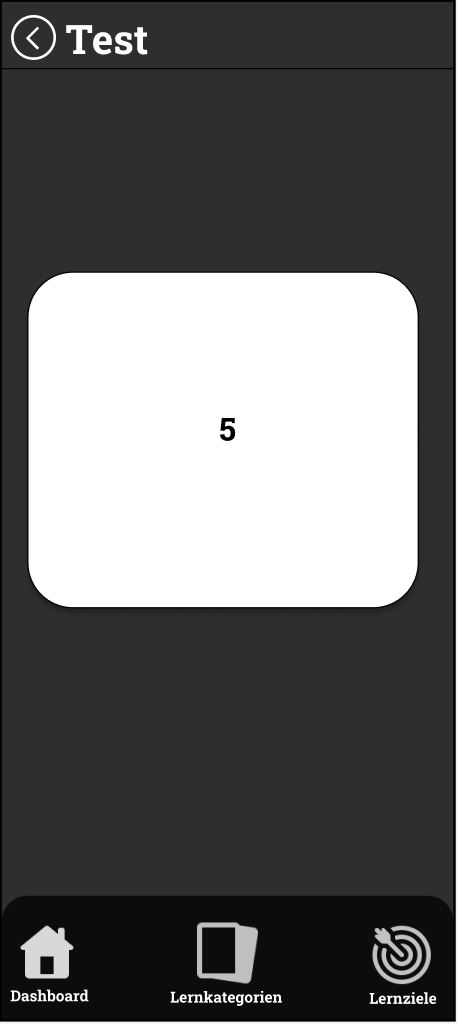
\includegraphics[width=\linewidth]{images/Mockups/TestAntwort.JPG}
    \caption{Ansicht einer Antwort innerhalb eines Tests}
    \label{fig:test-antwort}
  \end{subfigure}
  \hfill
  \begin{subfigure}[b]{0.45\linewidth}
    \centering
    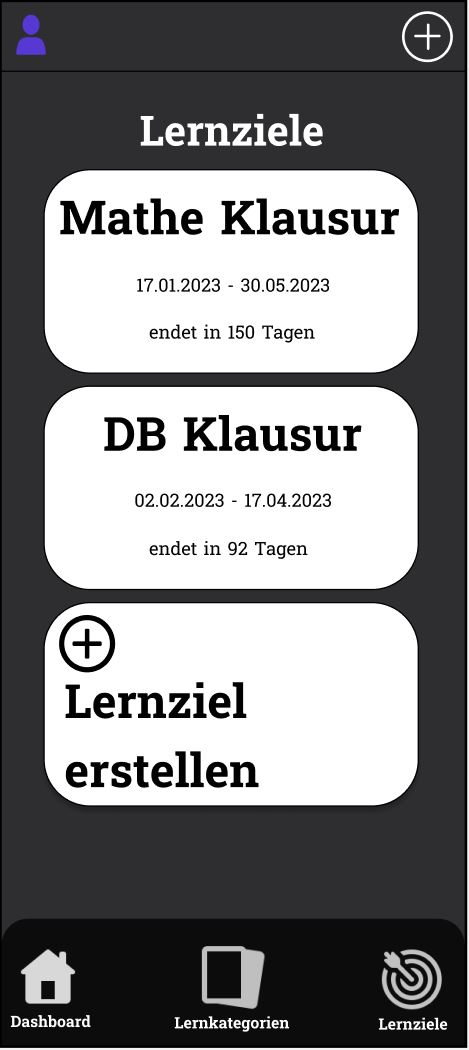
\includegraphics[width=\linewidth]{images/Mockups/Lernziele.JPG}
    \caption{Ansicht Lernziele}
    \label{fig:lernziele}
  \end{subfigure}
  \caption{Test}
\end{figure}

\newpage

\begin{figure}[H]
  \centering
  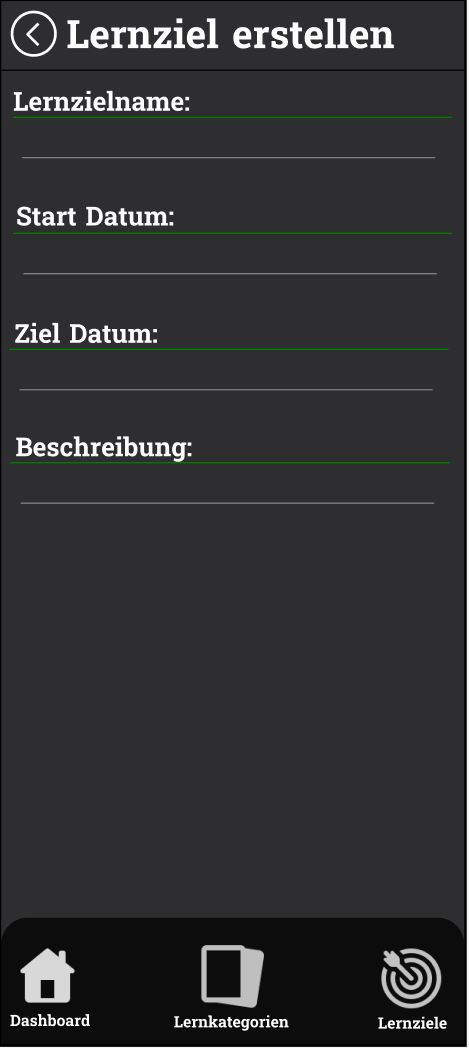
\includegraphics[width=0.5\linewidth]{images/Mockups/LernzielErstellen.JPG}
  \caption{Erstellen eines Lernziels}
  \label{fig:lernziel-erstellen}
\end{figure}

\newpage

\subsection{Datenflussdiagramm}
  \section{Entwurf}
\subsection{Geschäftsfälle anhand des BPMN Workflows}
\subsection{Auswahl und Begründung des Datenbankkonzepts}
Die Lern-App \gqq{LearnAhead} benötigt eine Datenbank, um die Lerninhalte des Benutzers speichern zu können. Die Datenbank soll hierbei die folgenden Anforderungen erfüllen:
\begin{itemize}
    \item Es soll möglich sein, Bilder einfach zu speichern und abzurufen.
    \item Die Datenbank soll gut skalierbar sein, um auch bei vielen Benutzern eine gute Performance zu gewährleisten.
    \item Es müssen gute Frameworks zur Anbindung für die Sprache Kotlin existieren.
    \item Die Datenbank soll in der Cloud gehostet werden, um die Wartungskosten zu minimieren.
    \item Die Datenbank soll möglichst kostenlos sein.
\end{itemize}

\noindent
Hierbei gab es die Entscheidung zwischen einer relationalen und einer NoSQL Datenbank. Da diese für die Speicherung von Bildern zuständig ist, ist eine NoSQL Datenbank die bessere Wahl. In diesem Zusammenhang kam der Anbieter \gqq{Firebase} in Frage. Dieser bietet zwei unterschiedliche Datenbanken an: \gqq{Cloud Firestore} und \gqq{Realtime Database}. Realtime Database wird genutzt, wenn die Datenbank in Echtzeit synchronisiert werden soll. Da dies bei der Lern-App nicht notwendig ist, wurde sich für Cloud Firestore entschieden. Cloud Firestore baut auf den Erfolgen von Realtime Database auf und bietet zusätzlich eine bessere Skalierbarkeit und ermöglicht zudem schnellere Abfragen. \cite*{Firestore} Für die Speicherung von Inhalten gibt es den Firebase Storage, welcher eine einfache Möglichkeit bietet, Inhalte wie z.B. Bilder oder Videos zu speichern. \newline

\noindent
Firebase bietet eine gute Anbindung für Kotlin (siehe \ref*{Auswahl der Klassenbibliotheken/Frameworks}). Zusätzlich ist Firebase kostenlos, solange die Datenbank nicht zu groß wird. Hierbei kann eine monatliche Anzahl von 50.000 Nutzern, 20.000 Schreibvorgängen und 50.000 Lesevorgängen kostenlos genutzt werden. Der Speicherplatz für den Firebase Storage beträgt 1 GB, welcher für die Lern-App ausreichend ist. \cite*{Firebase_Pricing}
\subsection{Auswahl der Klassenbibliotheken/Frameworks} \label{Auswahl der Klassenbibliotheken/Frameworks}
\subsection{Design Patterns für relevante Problemstellungen} \label{Design Patterns für relevante Problemstellungen}
\subsection{Software-Komponenten}
Das System wird zunächst als Gesamtkomposition dargestellt. Anschließend werden die Subsysteme einzeln dargestellt. 
\subsubsection{Gesamtkomposition}
\begin{figure}[H]
    \centering
    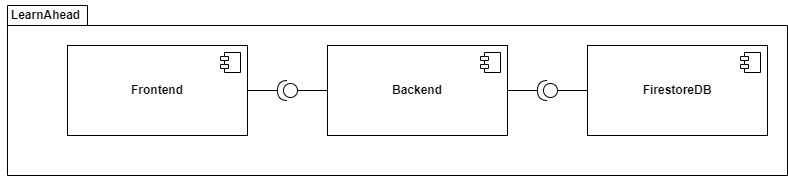
\includegraphics[width=0.8\textwidth]{images/diagramme/Gesamtkomposition.png}
    \caption{Gesamtkomposition}
    \label{fig:Gesamtkomposition}
\end{figure}
\noindent
Die Gesamtkomposition besteht aus den folgenden Subsystemen:
\begin{itemize}
    \item \textbf{Frontend:} Das Frontend ist für die Darstellung der Benutzeroberfläche zuständig. Es kommuniziert mit dem Backend, um Daten anzuzeigen und Eingaben an dieses weiterzuleiten.
    \item \textbf{Backend:} Das Backend ist für die Verarbeitung und Validierung der Daten zuständig. Es kommuniziert mit der FireStore Datenbank, um Daten abzurufen und zu speichern.
    \item \textbf{FireStoreDB} Die FireStoreDB Komponente ist die Datenbank-Komponente.
\end{itemize}

\noindent
Näheres hierzu im Deployment Diagramm \ref*{Deployment Diagramm} und Klassen Diagramm \ref*{Klassen Diagramm}.
\newpage
\subsubsection{Frontend}
Es gibt zwei Diagramme für das Frontend. Das Diagramm \ref*{fig:FrontendUINavigation} zeigt die Navigation zwischen den einzelnen Pages.
\begin{figure}[H]
    \centering
    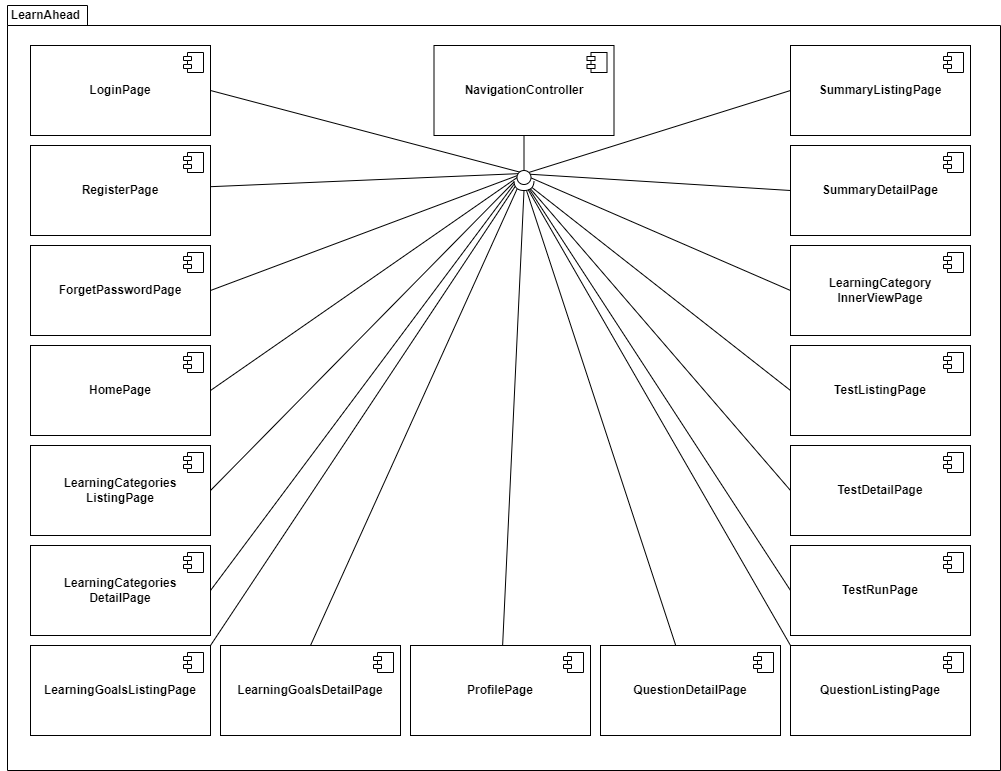
\includegraphics[width=0.8\textwidth]{images/diagramme/FrontEndKomposition.png}
    \caption{Frontend UI Navigation}
    \label{fig:FrontendUINavigation}
\end{figure}
\noindent
Das Diagramm \ref*{fig:FrontendUIViewModel} zeigt die Kommunikation zwischen den einzelnen Pages und dem ViewModel. Hierbei ist zu beachten, dass dieses Diagramm die Kommunikation zwischen den einzelnen Pages und dem ViewModel im Allgemeinen zeigt. Das bedeutet, dass jede Page ein zugehöriges ViewModel hat. Die Kommunikation zwischen den einzelnen Pages und dem ViewModel ist prinzipiell immer gleich. Weitere Details sind in Kapitel \ref*{Design Patterns für relevante Problemstellungen} zu finden. \newline
\begin{figure}[H]
    \centering
    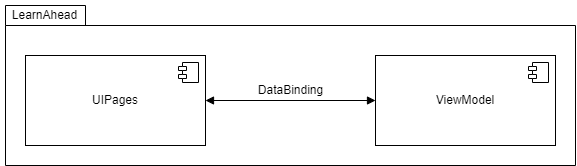
\includegraphics[width=0.8\textwidth]{images/diagramme/UIPagesMitViewModel.png}
    \caption{Frontend UI Kommunikation mit ViewModel}
    \label{fig:FrontendUIViewModel}
\end{figure}
\subsubsection{Backend}
Das Diagramm \ref*{fig:BackendKomposition} zeigt die Komposition des Backends. Hierbei ist zu beachten, dass dieses Diagramm die Komposition des Backends im Allgemeinen zeigt. Jedes Objekt, welches in der Datenbank gespeichert wird, hat ein zugehöriges Repository/Model. Die Kommunikation zwischen den verschiedenen Repositories und Modellen verläuft grundsätzlich immer auf die gleiche Weise. Jedes Repository baut auf einem Interface auf, welches die grundlegenden Funktionen für die Kommunikation mit der Datenbank definiert. Die Kommunikation mit der Datenbank erfolgt über das Repository.
\begin{figure}[H]
    \centering
    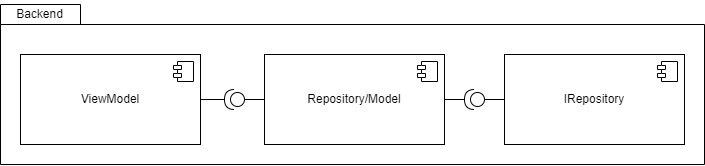
\includegraphics[width=0.8\textwidth]{images/diagramme/Backend.png}
    \caption{Backend Komposition}
    \label{fig:BackendKomposition}
\end{figure}
\subsection{Deployment Diagramm} \label{Deployment Diagramm}
\subsection{Klassen Diagramm} \label{Klassen Diagramm}
\subsection{Aktivitätsdiagramm}
\subsection{Sequenzdiagramme}
\subsection{Prototyp (optional)}
  \section{Ergebnisse}
Im folgenden Kapitel werden die Ergebnisse unserer Lern-App präsentiert und aufgelistet.
\subsection{Nutzen der Lern-App}
Der Nutzen unserer geplanten und dahingehend entwickelten Lern-App LearnAhead liegt darin die Studierenden der DHBW bei ihrem Lernprozess zu unterstützen.\\

\noindent
Es können nicht nur Lerninhalte in eine Lernkategorie kategorisiert, sondern auch, mit Hilfe der Lernziele, ihr Zeitlicher Rahmen erfasst werden.\\

\noindent
Die Lerninhalte können mit den Zusammenfassungen einer Lernkategorie mit dem Markdown-Editor erfolgreich erfasst und kondensiert werden.\\
Zu diesen Lerninhalten kann man dann Tests und Fragen erstellen, welche sich auf diese beziehen.

\subsection{Feedback von Präsentation der Studienarbeit}
Im Rahmen der Studienarbeiten wurde uns am 25.05.2023 die Möglichkeit geboten unsere Studienarbeiten in den Räumen N001 bis N004 im Rahmen eines Plakat Forums vorzustellen. \\

\noindent
Hierbei wurde unter anderem die Idee für das weiterreichen der Lerninhalte gegeben, da diese momentan noch von Hand eingegeben werden müssen.\\

\noindent
LearnAhead stoß auf großes Interesse und es wurde vieles hinterfragt, was uns noch umso mehr Ideen einbrachte, von denen einige in den Ausblick wanderten, da die Möglichkeiten bei der Entwicklung einer Lern-App praktisch unendlich sind. Mehr dazu siehe Kapitel \ref{sec:Ausblick}.

\newpage
\subsection{Der finale Zeitplan}
Im Folgenden findet sich der finale Zeitplan, so wie er zum Schluss umgesetzt wurde.\\
\begin{table}[H]
  \centering
  \resizebox{\columnwidth}{!}{%
  \begin{tabular}{l|l|l}
  \multicolumn{1}{c|}{\textbf{Meilenstein}} &
    \multicolumn{1}{c|}{\textbf{Zeitplan}} &
    \multicolumn{1}{c}{\textbf{Beschreibung}} \\ \hline
  Literaturrecherche &
    \begin{tabular}[c]{@{}l@{}}14.10.2022 - \\ 31.01.2023\end{tabular} &
    \begin{tabular}[c]{@{}l@{}}Das Durchführen einer umfangreichen Literaturrecherche\\ auf Basis von wissenschaftlichen Dokumenten.\end{tabular} \\ \hline
  Use-Case-Erstellung &
    \begin{tabular}[c]{@{}l@{}}14.10.2022 - \\ 11.11.2022\end{tabular} &
    \begin{tabular}[c]{@{}l@{}}Identifizierung und Dokumentation der \\ Hauptfunktionalitäten und Anwendungsfälle der Lern-App.\end{tabular} \\ \hline
  UI-Konzept &
    \begin{tabular}[c]{@{}l@{}}11.11.2022 - \\ 02.02.2023\end{tabular} &
    \begin{tabular}[c]{@{}l@{}}Entwicklung eines visuellen Konzepts für die \\ Benutzeroberfläche (UI) der Lern-App.\end{tabular} \\ \hline
  Datenbank-Konzept &
    \begin{tabular}[c]{@{}l@{}}20.01.2023 - \\ 16.02.2023\end{tabular} &
    \begin{tabular}[c]{@{}l@{}}Design und Auswahl des Datenbanksystems, die für die \\ App benötigt wird.\end{tabular} \\ \hline
  Architektur-Konzept &
    \begin{tabular}[c]{@{}l@{}}03.02.2023 -\\ 16.02.2023\end{tabular} &
    \begin{tabular}[c]{@{}l@{}}Realisierung einer Code-Architektur und Auswahl  \\ verschiedener Komponenten sowie Framekworks, \\ die in der App verwendet werden.\end{tabular} \\ \hline
  Architektur-Prototyp &
    \begin{tabular}[c]{@{}l@{}}10.02.2023 - \\ 16.02.2023\end{tabular} &
    \begin{tabular}[c]{@{}l@{}}Erstellung eines ersten Prototypen \\  der die vorgeschlagene Architektur implementiert.\end{tabular} \\ \hline
  Login / Registrierung &
    \begin{tabular}[c]{@{}l@{}}17.02.2023 - \\ 30.03.2023\end{tabular} &
    \begin{tabular}[c]{@{}l@{}}Implementierung der Funktionen für Anmeldung, \\ Registrierung und Passwortwiederherstellung.\end{tabular} \\ \hline
  \begin{tabular}[c]{@{}l@{}}Lernkategorien \& \\ Lernziele\end{tabular} &
    \begin{tabular}[c]{@{}l@{}}31.03.2023 -\\ 11.05.2023\end{tabular} &
    \begin{tabular}[c]{@{}l@{}}Implementierung der Funktion zum Erstellen sowie Verwalten\\  von Lernkategorien und -zielen.\end{tabular} \\ \hline
  \begin{tabular}[c]{@{}l@{}}Erstellung von Fragen \\ und Tests\end{tabular} &
    \begin{tabular}[c]{@{}l@{}}12.05.2023 -\\ 11.07.2023\end{tabular} &
    \begin{tabular}[c]{@{}l@{}}Implementierung der Funktion zum Erstellen sowie Verwalten\\  von Fragen und Tests.\end{tabular} \\ \hline
  \begin{tabular}[c]{@{}l@{}}Erstellung von \\ Zusammenfassungen\end{tabular} &
    \begin{tabular}[c]{@{}l@{}}12.05.2023 -\\ 11.07.2023\end{tabular} &
    \begin{tabular}[c]{@{}l@{}}Implementierung der Funktion zum Erstellen sowie  \\ Verwalten von Zusammenfassungen von Lernkategorien.\end{tabular} \\ \hline
  \begin{tabular}[c]{@{}l@{}}Optimale Pausenberechnung \\ realisieren\end{tabular} &
    \begin{tabular}[c]{@{}l@{}}12.07.2023 -\\ 14.07.2023\end{tabular} &
    \begin{tabular}[c]{@{}l@{}}Erstellung eines Algorithmus, welcher den Nutzer die  \\ optimale Pause vorschlägt sowie errinert.\end{tabular} \\ \hline
  \begin{tabular}[c]{@{}l@{}}Optimale Lernplan \\ generieren\end{tabular} &
    \begin{tabular}[c]{@{}l@{}}12.07.2023 -\\ 14.07.2023\end{tabular} &
    \begin{tabular}[c]{@{}l@{}}Erstellung eines optimalen Lernplans auf Basis der Lernziele.\\\end{tabular} \\ \hline
  Durchführen von User-Tests &
    \begin{tabular}[c]{@{}l@{}}09.07.2023 -\\ 16.07.2023\end{tabular} &
    \begin{tabular}[c]{@{}l@{}}Durchführung von umfassenden Tests, um die Qualität, \\ Funktionalität und Stabilität der App sicherzustellen.\end{tabular} \\ \hline
  Bugs beheben &
    \begin{tabular}[c]{@{}l@{}}14.07.2023 - \\ 16.07.2023\end{tabular} &
    \begin{tabular}[c]{@{}l@{}}Behebung von Fehlern und Problemen in der App.\end{tabular} \\ \hline
  Dokumentation &
    \begin{tabular}[c]{@{}l@{}}14.10.2022 - \\ 16.07.2023\end{tabular} &
    \begin{tabular}[c]{@{}l@{}}Erstellung einer wissenschaftlichen Arbeit, die das Vorgehen, \\ Funktionen, die Implementierung sowie die Verwendung \\ der App begründet.\end{tabular}
  \end{tabular}%
  }
  \end{table}

  \noindent
  Anhand des finalen Zeitplans lässt sich erkennen, dass die Implementierung von den Zusammenfassungen, Fragen und Tests mehr Zeit in Anspruch genommen hat, als ursprünglich geplant. Daraus folgt, dass das \gqq{Springen} mithilfe von Tags nicht mehr implementiert werden konnte.
  %%%%%%%%%%%%%%%%%%%%%%% Literaturverzeichnis %%%%%%%%%%%%%%%%%%%%%%%
  \printbibliography[title=Referenzen]
\addcontentsline{toc}{section}{Referenzen}
\newpage


  %%%%%%%%%%%%%%%%%%%%%%%%%%%%%% Anhang %%%%%%%%%%%%%%%%%%%%%%%%%%%%%%
  \renewcommand{\thetable}{\Alph{section}.\arabic{table}}
  \renewcommand{\thefigure}{\Alph{section}.\arabic{figure}}
  \renewcommand{\thelstlisting}{\Alph{section}.\arabic{lstlisting}}
  \pagenumbering{Alph}

  \begin{appendix}
  \section{Anhang}




\end{appendix}
\end{document}